\section{Introduction}

The Description of Work describes Task 3.3 thus
\begin{quote}
Task 3.3: Develop tools and techniques to model, in an uniform way, the differences between different versions of
a system, which are parametrized or configured in different ways.
\end{quote}

\subsection{Behaviour refactoring}

The abstraction principle tells us that we must not repeat code. As
stated by \cite{pierce2002types} ``Each significant piece of functionality
in a program should be implemented in just one place in the source
code. Where similar functions are carried out by distinct pieces of
code, it is generally beneficial to combine them into one by abstracting
out the varying parts''. In practice we cannot always see what abstraction
we need until we have already replicated code. 

Having replicated code is bad because it forces us to make modifications
to the replicated code several times. We will eventually forget to
modify all the instances and we will go from having replicated code,
to having one subset of the bugs solved in one of the instances, and
another subset of them in the other one.

Erlang provides a mechanism for abstracting and parametrising implementations
at module level: \emph{Erlang behaviours}. A behaviour is given by a module in which 
some function definitions are missing: these functions provide a \emph{callback interface}. A module
implementing this interface is called an \emph{instance} of the behaviour.

In this work we study a set of mechanisms to automatically assist developers in the creation of Erlang behaviours in 
an incremental way, as well as showing how to ``unfold'' a behaviour and an instance of it into a single module. We 
also show how a behaviour can be inferred and created  from two modules with similar implementations. All of the 
refactorings described here are available as part of the open-source refactoring tool Wrangler, and make use of the 
Wrangler API and DSL that facilitate user-defined extensions of the tool. 

In many application areas, system variants are prevalent, and so multiple models are developed, which differ in some 
aspects of behaviour but share overall structure as well as most aspects of behaviour. In such a situation, it is 
desirable to develop parametric models, and the work reported here supports building parametrised models from existing 
variants. It is worth emphasizing again that this is \emph{parametrisation over 
functionality}, and not simply over 
data, and so provides a general parametrisation framework.


\subsection{Erlang behaviours\label{sec:erlang_behaviours}}

\emph{Erlang Behaviours} are a standard Erlang mechanism that allows the
parametrisation of modules. A \emph{behaviour} is composed of two parts: a behaviour definition and one or more behaviour instances.


A \textbf{behaviour definition} is an Erlang module that defines a series of callbacks
that its \emph{behaviour instances} must implement. This can be done
in one of two ways:

\begin{itemize}
\item Through \texttt{-callback} declarations, which specify the expected
callbacks and their type signatures. For example:
{\small
\begin{verbatim}
-callback terminate(Reason :: (normal | shutdown |
                               {shutdown, term()} |
                               term()),
                    State :: term()) -> term().
\end{verbatim}
}

\item Through a \texttt{behaviour\_info/1} function that specifies the name
and arity of the expected callbacks. For example:
{\small
\begin{verbatim}
behaviour_info(callbacks) ->
                 [{init, 1}, {handle_call, 3},
                  {handle_cast, 2}, {handle_info, 2},
                  {terminate, 2}, {code_change, 3}];
behaviour_info(_) -> undefined.
\end{verbatim}
}
\end{itemize}

In this work we have only considered the \texttt{behaviour\_info/1}
function because, currently, there is limited support for \texttt{-callback}
declarations by the abstract syntax tools. These two approaches are
mutually exclusive, the Erlang compiler will complain if both are
used at the same time. The work reported here can be extended to the \texttt{-callback}
declaration approach in a straightforward way, given a specification of the type(s) of the function(s)
in question, which can come either from the user -- who might indeed have declared types for the functions 
already -- or using dialyzer/typer type inference. 

Each \textbf{behaviour instance} is an Erlang module that must implement the callbacks
defined by the \emph{behaviour definition} and contain a \texttt{behaviour}
declaration that specifies which \emph{behaviour definition} they
implement. 

A behaviour instance will be an Erlang module containing a \texttt{behaviour} declaration of the form:\begin{verbatim}
-behaviour(gen_server).
\end{verbatim}
together with definitions of the callback functions, as well as definitions of any other relevant functions.

\subsection{Wrangler usage}\label{wrangler-usage}

The refactorings for manipulation of Erlang behaviours presented here can be understood, to a large extent, in terms of 
smaller existing refactorings. Because of that, we have been able to reuse a lot of functionality that was already 
available in Wrangler. In particular, the refactorings that assist the iterative manipulation of Erlang behaviours have 
been implemented by using Wrangler's DSL for composite refactorings.

Several of the primitive refactorings, used by the new composite refactorings, already existed. Some of the 
new refactorings were created through the use of the API for user-defined refactorings, and even some of the 
refactorings that were created as internal extensions to Wrangler were based on 
existing ones. For example, the new copy module refactoring was based on the 
existing rename module refactoring. For this reason, the work described in this 
deliverable validates the effectiveness of Wrangler's DSL for extending the applicability of Wrangler.

The refactoring for automatic behaviour extraction was implemented in its entirety as an internal extension to 
Wrangler, but both the internal infrastructure and the refactoring API were used extensively. This support allowed the 
new implementations to inherit properties like code layout and comment preservation.

Finally, low-level mechanisms provided by Wrangler, (like the categorisation of AST nodes, or the module information 
extraction), have already been extensively tested in production settings. Being able to reuse these mechanisms grants 
our implementation with an increased level of safety that would be costly to achieve with an implementation from 
scratch.

The branch of Wrangler containing these extensions and the code for case studies is available at 
\url{https://github.com/RefactoringTools/wrangler}, (branch draft-release-1.2).

\subsection{Extended Finite State Machine Inference}

The previous components of this work package have included various applications of Finite State Machine Inference \cite{d31,d32}. This was shown to be a powerful and valuable technique for both understanding the behaviour of a particular system, and capturing and visualising the differences between versions of systems. However, since Finite State Machines (FSMs) model systems as a series of states with atomic events transitioning between them they are incapable of modelling parameterised systems whose behaviour is dependent on data (at least for a practical limit on the number of states).

Extended Finite State Machines (EFSMs) \cite{EFSMs} extend the atomic transitions of FSMs to include parameters on the events, data registers within the state, guard expressions over the data state, and update functions to modify the data state. Taking the existing, successful work on inferring FSMs and using them to model behaviour differences, and extending this to EFSMs was a natural way to apply this work to parameterised systems.

Inferring EFSMs has several additional complexities over inferring FSMs, since not only the \emph{control flow} states of the system, but also the composition and use of the \emph{data state} must be considered. Previous expertise developed at USFD, in conjunction with other researchers \cite{NeilEFSMs}, was leveraged to allow a prototype inference tool to be developed within the timeframes of this task. The open-source Athena tool \cite{Athena} has been constructed and released as a prototype to demonstrate the feasibility and value of EFSM inference for understanding parameterised systems.

By applying EFSM inference to different versions of parameterised systems produces models that include the differences in the parametric or data-driven behaviours. This demonstrates the potential to apply differencing and visualisation techniques to these extended models, in a similar way to their application to finite state models in previous deliverables \cite{d31,d32}. 

\section{Related Work}
\label{related_work}
\label{sec:related_work}

\paragraph{Abstraction introduction}

Existing refactoring tools for object-oriented languages (including IntelliJ IDEA, Eclipse and NetBeans) provide 
a facility to extract an interface from OO code. The closest to the work we report here is the IntelliJ IDEA 
implementation, 
in which the third option \emph{``rename[s] the original class, [so that] it implements the newly created 
interface.''}~\cite{intellij-extract}. Our work differs from this in being tuned to work particularly with Erlang code, 
and also in supporting the incremental development of the behaviour, one function at a time. It also supports the 
automated identification of possibilities for interface introduction, which is also not supported in the implementations 
for other languages.

\paragraph{Behaviour identification}

Our approach has a lot in common with clone detection. The main difference
is that in this approach we assume that we know the root of the replication
and we are actually finding the different parts, and clone detection
assumes that most of the code is different and tries to find the commonalities.
In our case we assume that we start with two modules which are similar
and we try to find a common structure between both and create an Erlang
behaviour. For this reason the problem is not so much locating the
common parts but matching them appropriately. Thus, in our case it
makes more sense to explore structural commonalities in depth, whereas
in clone detection it is often more effective to focus on the sequential
behaviour.


The previous work that we have found which is most similar to the
one presented here is \cite{chawathe1996change}, which strongly
inspired this work. Tree comparison has been researched extensively
\cite{bille2005survey}, a big part targeted at XML \cite{peters2005change}.
Of course, the nature of XML is quite different to the one of Erlang,
but they both share the use of nested structures and semi-structured data.

\paragraph{Clone detection}

There is an extensive literature on software clones: \cite{Roy07Survey} surveys work in the area up to 2007, and there 
is also a regular \emph{International Workshop on Software Clones}~\cite{IWSC10,IWSC11}. While some code clones might 
have a sound reason for their existence~\cite{KasperGodfrey06,Cordy2003}, many clones are considered to be detrimental 
to the quality of software, because code duplication makes it more likely that  bugs will be propagated, as well as 
increasing the size of the source
code and the executable, the compile time, and most importantly the overall cost of maintenance~\cite{Monden02}.

The existing body of work on software clones places an emphasis on clone identification, analysis and classification -- 
both theoretical and practical~\cite{TowardsTaxonomy} -- as well as on the evolution and tracking of clones during the 
lifetime of a project. This literature encompasses theoretical work on different mechanisms of clone identification, as 
well as case studies that  show the presence of code clones in most projects, typically accounting for at least ten 
percent of the existing code base.



\section{Assisted behaviour creation and unfolding with Wrangler}
\label{sec:assisted-creation}

In order to prevent code replication, it is usually possible and
convenient to abstract and parametrise those common parts of the implementation
into a single location, (typically another module), that can be invoked
from each of the individual, (not common), parts. Unfortunately, taking
this precaution requires an additional initial effort which may deter
developers from adopting it, in situations where time is limited.

We claim that this process can be automated to a large extent. By
introducing automation, we intend to help reduce the friction and
the likelihood of errors being introduced and, as a consequence, we
expect that parametrisation will be used more broadly as a replacement
for replication.

\subsection{Overview}

In this work we present a series of new refactorings for Wrangler tool
\cite{li2008refactoring}, which automate the creation and unfolding of Erlang
\emph{behaviour instances} (see Section~\ref{sec:erlang_behaviours}).
The refactorings are mostly written using Wrangler's \emph{DSL for composite
refactorings} \cite{li2012domain} and \emph{callback interface for
user-defined refactorings} \cite{li2011user}, but some parts were implemented
as internal extensions to Wrangler.

The main functionality can be summarised as follows:
\begin{itemize}
\item Creation of a single Erlang \emph{behaviour instance} from either:

\begin{itemize}
\item An existing function in a module
\item An expression in a module
\end{itemize}
\item Unfolding of a single \emph{behaviour instance} against its \emph{behaviour
definition}
\end{itemize}


\subsection{\emph{Behaviour} extraction\label{sec:behaviour-extraction}}

\emph{Behaviour} extraction creates a new \emph{behaviour callback} from an existing
piece of code, and it moves the code to a new or existing \emph{behaviour instance} so
that it is used by the \emph{behaviour instance} to implement the new
\emph{behaviour callback}.

It is supported by two alternative composite refactorings: \emph{Expression
to behaviour instance} and \emph{Function to behaviour instance}. Both
behave similarly, but the first one expects the user to select an expression
and it will automatically apply \emph{Function Extraction} to the expression
before the \emph{behaviour} instantiation. The second one assumes that the
behaviour callback implementation that must be extracted is already in a
separate function, and expects the user to select it.

Either way, the selected function will be moved to a new or existing
module (the \emph{behaviour instance}). The refactoring will ensure
that a \texttt{behaviour\_info/1} function is created if it does not
exist, and that the function moved is added to the \texttt{behaviour\_info/1}
function. It will also ensure that the \texttt{behaviour} declaration
is added to the \emph{behaviour instance} if it does not have it already. 

Internally, the composite refactorings call the following individual
refactorings in order:
\begin{itemize}
\item \emph{Create behaviour instance file} --- creates the \emph{behaviour
instance} if it does not exist. It prompts for the name of the module
to contain the \emph{behaviour instance} (see Section~\ref{sub:create_behav_instance})
\item \emph{Function Extraction} (only for \emph{Expression to behaviour
instance}) --- creates a new function with the selected expression.
It prompts for a name for the new function. No function with the provided
name should exist in the \emph{behaviour instance} nor the \emph{behaviour
declaration} (see Section~\ref{sub:fun_extraction})
\item \emph{Add function to behaviour\_info} --- adds the function to the
list of callbacks to implement by \emph{behaviour instances} (see
Section~\ref{sub:add_callback})
\item \emph{Move Function to Another Module} --- moves the implementation
of the function to the \emph{behaviour instance} (see Section~\ref{sub:move_fun})
\end{itemize}
A limitation of this process is that the generated calls to the functions
added to the \emph{behaviour instances} are statically targeted to
the specified \emph{behaviour instance}. For example, a call will have the
form \texttt{server:start()} where \texttt{server} is the name of
the \emph{behaviour instance} we just extracted, instead of \texttt{Module:start()}
where \texttt{Module} is a variable. For the \emph{behaviour} to
be able to use several \emph{behaviour instances}, it is necessary
that these static calls are generalised somehow.

For some scenarios, one way around this starts by using the existing
refactoring \emph{Generalise Function Definition} while selecting
the module name of the \emph{behaviour instance} used (this is explained
in more detail in Section~\ref{sub:adjustments-for-generalisation}).

We decided not to automate this process because it depends heavily
in the particular scenario, and multiple alternative possibilities
for the parametrisation are possible, (e.g: the definition of a macro,
or the inclusion of a variable in the state of a process, see 
Section~\ref{sub:alternative-adjustments-for-generalisation}).


\subsection{\emph{Behaviour} unfolding\label{sec:behaviour-unfolding}}

\emph{Behaviour} unfolding aims to reverse the process of \emph{behaviour}
extraction, i.e: the specific code in the \emph{behaviour instance}
is combined with a copy of the generic code in the \emph{behaviour
declaration}. A copy is made in order to ensure other \emph{behaviour
instances} keep working. This process is supported by the composite
refactoring \emph{Unfold behaviour instance}. This refactoring must
be called from the \emph{behaviour instance} to unfold and it takes
as input the name of the destination module.

The composite refactoring internally calls the following individual
refactorings in order:
\begin{itemize}
\item \emph{Copy module} --- copies the \emph{behaviour definition} to the
destination module name while updating only the references from the
current \emph{behaviour instance} (see Section~\ref{sub:copy_mod})
\item \emph{Instantiate calls} (optional step) --- instantiates the dynamic
calls with function names that match the \emph{behaviour} interface
in the new copy \emph{behaviour definition}, i.e: it will modify the
qualified calls whose module is not hard-coded by setting their target
module to the particular \emph{behaviour definition} specified (see
Section~\ref{sub:instantiate_calls})
\item \emph{Move function} --- moves the functions from the \emph{behaviour
instance} to the new copy of the \emph{behaviour definition} (see
Section~\ref{sub:move_fun})
\item \emph{Remove behaviour declaration} --- removes the \texttt{behaviour\_info/1}
function from the new copy of the \emph{behaviour definition} (see
Section~\ref{sub:remove_behav_dec})
\end{itemize}
A limitation of this process is that \emph{Instantiate calls} is only
an approximate solution to the problem of dynamic calls. Even though
this refactoring will instantiate the right calls correctly in the
majority of scenarios, it will not remove unused variables.

These variables must be removed by hand or else they will usually
produce compilation warnings, and clutter the code. In addition, in
the few cases where there may be dynamic calls to functions in other
modules, (i.e: not part of the \emph{behaviour}), with names that
match the ones in the \emph{behaviour} interface, the instantiation
may produce wrong results.

In these cases, the \emph{Instantiate calls} refactoring may be executed
individually, and each individual instantiation can then be checked
manually.

In some cases the \emph{Instantiate calls} refactoring may not be
necessary because the \texttt{?MODULE} macro is used for dynamic calls.
In these cases its application can be skipped by answering ``no''
when asked by the \emph{Unfold behaviour instance} refactoring about
instantiating dynamic calls.


\subsection{Basic refactorings}

In this section we provide an overview of the user-defined and primitive
refactorings used by the composite refactorings described in 
Sections~\ref{sec:behaviour-extraction}~and~\ref{sec:behaviour-unfolding}.


\subsubsection{Copy module\label{sub:copy_mod}}

This refactoring is based on the existing refactoring \emph{Rename
module}, and, as such, it was implemented as a primitive refactoring.
It will copy a module and update the external references to that module.
Unlike in the case of \emph{Rename module}, (where it would not make
sense), with \emph{Copy module} we can specify the list of modules
whose references we want to update. This way, the rest of modules
would keep pointing at the old version.


\subsubsection{Create \emph{behaviour instance} file\label{sub:create_behav_instance}}

This refactoring was implemented as an user-defined refactoring. It
takes as input a target module name. It creates a file for the module
if it does not exist, and it adds a \texttt{behaviour} declaration
to the file if it does not have it.


\subsubsection{Add function to \texttt{behaviour\_info/1}\label{sub:add_callback}}

This functionality was actually implemented as two alternative refactorings:
\begin{itemize}
\item \emph{Add function to behaviour\_info} --- adds a single pair \texttt{\{FunctionName,
Arity\}} to \texttt{behaviour\_info}
\item \emph{Add function name to behaviour\_info} --- adds a pair for each
of the functions that are defined in the module and have the name
specified, (i.e: independently of their arity)
\end{itemize}
Both versions of the refactoring were implemented as user-defined
refactorings. Both create the \texttt{behaviour\_info} function if
it does not exist, and then add the functions specified to the list
of callbacks in it.

In order for the result of this refactoring to work, there must not
be any callback definitions in the \emph{behaviour definition} module.


\subsubsection{Remove \texttt{behaviour} declaration\label{sub:remove_behav_dec}}

This refactoring will search for the function \texttt{behaviour\_info/1}
and it will delete its implementation and remove it from every \texttt{export}
declaration in the module. If an \texttt{export} declaration only
contains that function, it will also be deleted.

It was implemented as an user-defined refactoring.


\subsubsection{Instantiate calls\label{sub:instantiate_calls}}

This refactoring tries to instantiate dynamic calls that target functions
of the \emph{behaviour} interface. It does so by searching for qualified
function calls with a target function name that corresponds to a function
from the \emph{behaviour} interface but with a module that is not
defined by an atom, (e.g: defined by a variable or a macro). And it
replaces the module with the name of the \emph{behaviour instance}
provided.

It was implemented as an user-defined refactoring.


\subsubsection{Move Function to Another Module\label{sub:move_fun}}

This refactoring was already part of Wrangler. It takes a function
and moves it with its local dependencies to a different module while
ensuring that all the references to the old function are updated.
It will also add the function to the list in the \texttt{export} declaration
if necessary.


\subsubsection{Function Extraction\label{sub:fun_extraction}}

This refactoring was already part of Wrangler. It takes an expression
an creates a new function for it. It also adds a parameter to the
function for each unbound variable within the expression.


\subsection{Example}

In this section we will go through a simple example of how the refactorings
described can be used to extract and unfold a \emph{behaviour instance}.


\subsubsection{Creating a \emph{behaviour} from scratch}

In Figure~\ref{fig:initial_code} we have provided a simple module
called \texttt{bar}. This module has two functions. The function \texttt{bar/0}
has the common behaviour, and the function \texttt{foo/0} has the
exclusive behaviour. In our case the exclusive behaviour is isolated
in a separate function, because of this we can set the cursor to point
to the function \texttt{foo/0} and use the refactoring \emph{Function
to behaviour instance}. If instead the function \texttt{bar/0} was
defined as follows:

\begin{verbatim}
bar() -> 42 + 1.
\end{verbatim}

We could still select the number 42, use the refactoring \emph{Expression
to behaviour instance}, and still obtain the same result.

\begin{figure}
\showcodeboxwithlabel{lst:initial_code}{figures/assisted_beh/code/step1/bar.erl}

\caption{Initial code\label{fig:initial_code}}
\end{figure}


When we execute the refactoring \emph{Function to behaviour instance},
we are asked about the ``Destination module'' which in our case
we called \texttt{new}. The refactoring will modify the module \texttt{bar}
to include the \texttt{behaviour\_info/1} function with our function
\texttt{foo/0} listed in it, and a new module \texttt{new} has been
created that contains the function \texttt{foo/0} and a \texttt{behaviour}
declaration that points to the module \texttt{bar}, 
(Figure~\ref{fig:after_ref}).

\begin{figure}
\begin{minipage}[t]{0.65\textwidth}%
\showcodehalfboxwithlabel{lst:bar_after_ref}{
figures/assisted_beh/code/step2/bar.erl
}%
\end{minipage}%
\begin{minipage}[t]{0.35\textwidth}%
\showcodeboxwithlabel{lst:new_after_ref}{figures/assisted_beh/code/step2/new.erl
}%
\end{minipage}

\caption{Behaviour definition and instance after 
extraction\label{fig:after_ref}}
\end{figure}



\subsubsection{Adjustments for 
generalisation\label{sub:adjustments-for-generalisation}}

As stated before, we can see that a limitation of the refactoring
is that the call to function \texttt{foo/0} in \texttt{bar/0} has
the module \texttt{new} hard-coded. This would be a problem if we
wanted to replicate the module \texttt{new} to generate more \emph{behaviour
instances}, (\texttt{bar} is not generic enough).

In order to solve this, we can generalise the call by, for example,
selecting the module qualifier \texttt{new} in \texttt{bar/0}, and
applying the refactoring \emph{Generalise Function Definition}, (in
our case with the parameter name \texttt{Module}), and then moving
the generated \texttt{bar/0} function to the module \texttt{new} by
using the refactoring \emph{Move Function to Another Module} twice,
(once to move \texttt{bar/0} to \texttt{new}, and once to bring \texttt{bar/1}
back to \texttt{bar} from \texttt{new}).

This procedure leaves us with the modules \texttt{bar} and \texttt{new}
shown in Figure~\ref{fig:manual_adj}.

\begin{figure}
\begin{minipage}[t]{0.6\textwidth}%
\showcodehalfboxwithlabel{lst:bar_manual_adj}{
figures/assisted_beh/code/step5/bar.erl}%
\end{minipage}%
\begin{minipage}[t]{0.4\textwidth}%
\showcodeboxwithlabel{lst:new_manual_adj}{
figures/assisted_beh/code/step5/new.erl}%
\end{minipage}

\caption{Behaviour definition and instance after adjustments for 
generalisation\label{fig:manual_adj}}
\end{figure}



\subsubsection{Alternative adjustments for 
generalisation\label{sub:alternative-adjustments-for-generalisation}}

The generalisation process described in 
Section~\ref{sub:adjustments-for-generalisation}
was not automated because it can be carried out by using several alternative
approaches which, in some cases, depend on the context of the implementation.
If the behaviour to use can be decided at compilation time it may
be generalised through the use of a macro (see 
Figure~\ref{fig:bar_manual_adj_b}).
\begin{figure}
\showcodeboxwithlabel{lst:bar_manual_adj_b}{
figures/assisted_beh/code/step5b/bar.erl}

\caption{Alternative adjustments for generalisation 
1\label{fig:bar_manual_adj_b}}
\end{figure}
If the behaviour represents a server, like is the case of \texttt{gen\_server},
the name of the \emph{behaviour instance} can be stored in the state
of the server or on the server dictionary (see 
Figure~\ref{fig:bar_manual_adj_c}).
\begin{figure}
\showcodeboxwithlabel{lst:bar_manual_adj_c}{
figures/assisted_beh/code/step5c/bar.erl}

\caption{Alternative adjustments for generalisation 
2\label{fig:bar_manual_adj_c}}
\end{figure}


Both alternatives remove the necessity of passing the name of the
\emph{behaviour instance} as a parameter. In exchange, the first approach
requires the decision to be taken at compilation time, (which is not
always possible), and the second one relies on side effects, (which
may eventually lead to integration errors that are harder to track).


\subsubsection{Unfolding a \emph{behaviour instance}}

For reverting the process we can call the refactoring \emph{Unfold
behaviour instance} from the \emph{behaviour instance} module. We
will be asked for a name to give to the resulting module, (in our
case we chose \texttt{bar\_new}), and whether we want to point all
dynamically-qualified callbacks to \texttt{new}. In our case we chose
\texttt{yes}, in order to revert the adjustments made in 
Section~\ref{sub:adjustments-for-generalisation}.

This will produce a module \texttt{bar\_new} like the one shown in
Figure~\ref{fig:unfold_result}.

\begin{figure}
\showcodeboxwithlabel{lst:unfold_result}{
figures/assisted_beh/code/step6/bar_new.erl}

\caption{Result of unfolding\label{fig:unfold_result}}
\end{figure}



\subsubsection{Removing spurious parameters}

We can see that both \texttt{bar/0} and \texttt{bar/1} in 
Figure~\ref{fig:unfold_result}
behave as \texttt{bar/0} in the Figure~\ref{fig:initial_code}, but
\texttt{bar/1} has a spurious parameter which will produce a warning.

For cleaner code we recommend manually removing the \texttt{bar/0}
function and transforming the function \texttt{bar/1} into \texttt{bar/0}
by removing the unused \texttt{Module} parameter, (whenever it is
unused, as is our case).

By doing this we will be left with the module \texttt{bar\_new} shown
in Figure~\ref{fig:final_result}.

\begin{figure}
\showcodeboxwithlabel{lst:final_result}{
figures/assisted_beh/code/step7/bar_new.erl}

\caption{Result of unfolding after removing spurious 
parameter\label{fig:final_result}}
\end{figure}

\section{Automatic behaviour identification with Wrangler}
\label{sec:identification}

When developing software, we might well realise that we should add
abstraction once we have implemented two pieces of similar
code. At this point, we must make an additional effort to find the
commonalities and unify them. This job is tedious and error prone,
and it does not provide any additional functionality, which makes
it difficult to justify. Nevertheless, it helps reduce maintenance
effort required in the future, and it will avoid the diversion in
the evolution of the code unified.

For this reason, in this section we study a mechanism that automatically
creates an Erlang behaviour by merging two modules selected by the
user, which are assumed to be structurally similar, and possibly the
result of copying and modifying one of them to produce the other.

This mechanism has been implemented and distributed as a refactoring
included in Wrangler refactoring tool for Erlang. Even though there is no
guarantee about this, since there may be bugs in the implementation and
the code could depend in complicated or conflicting macros which may
not be preserved correctly, the refactoring aims not to alter the behaviour
of the two modules targeted from the point of view of their external
interface, and it should only affect the organisation of the code
between the original modules, (which will be transformed by the refactoring
into \emph{behaviour instances}), and the newly created \emph{behaviour
definition}.

\subsection{Overview}

In general, the refactoring will only affect the organisation
of the code between the original modules, (which will be transformed by
the refactoring into \emph{behaviour instances}), and the newly created
\emph{behaviour definition}.

%\subsection{Overview}

The algorithm consists of three parts: tree matching 
(Section~\ref{sub:tree-matching}), cluster construction 
(Section~\ref{sub:cluster-cons}), and cluster linking 
(Section~\ref{sub:cluster-linking}). The process starts with two 
modules which are assumed to be similar. First we find commonalities between 
their ASTs,
group the contiguous commonalities, move the commonalities to a separate
module, and link the pieces together with function calls in order
to preserve the original behaviour. This way we are left with three
modules: the remains of the original ones and a new module with
the common parts.


\subsection{Tree matching\label{sub:tree-matching}}

In the first stage we apply a tree matching algorithm to find correspondences
between the ASTs, of both modules. In the current implementation we
have used the top-down tree matching algorithm described in \cite{al2005diffx},
because it is both easy to implement and effective. We have encapsulated
the tree matching algorithm in a way that would allow it to be replaced
easily by other algorithms in the future.

In particular, we have found some more recent and heavily tuned algorithms
that might be have been more appropriate for our approach
\cite{falleri2014fine,fluri2007change}, but we
discarded them because, due to their complexity, reimplementing them would
have been much more costly, and in the cases where there exist public
implementations of them, they are written in different languages, which
would have made the integration more difficult and cumbersome.

One specific consideration for applying tree matching to our problem is
deciding how to compare individual nodes of the syntax tree. We use
a simple dual approach:
\begin{itemize}
\item For \emph{leaf nodes}, which usually contain the semantic information, we
compare the literal representation of the nodes. This way, two variables
or two atoms are considered equal if and only if their names match.
It is important to remove any comments from the representation before
comparing, since these would produce false negatives.
\item For \emph{the other nodes}, which contain structural information, we 
compare
list constructors of the same length will be considered equal independently
list constructors of the same length will be considered equal independently
of their elements, but a tuple and a list of the same length, or two
lists of different lengths, will not.
\end{itemize}
Tree matching provides us with a mapping between equivalent nodes
from one AST to the other. In Figure~\ref{fig:tree-mapping-example}
we show what a possible tree mapping representation would look like,
where nodes with the same name are considered equal.

\begin{figure}
\centering
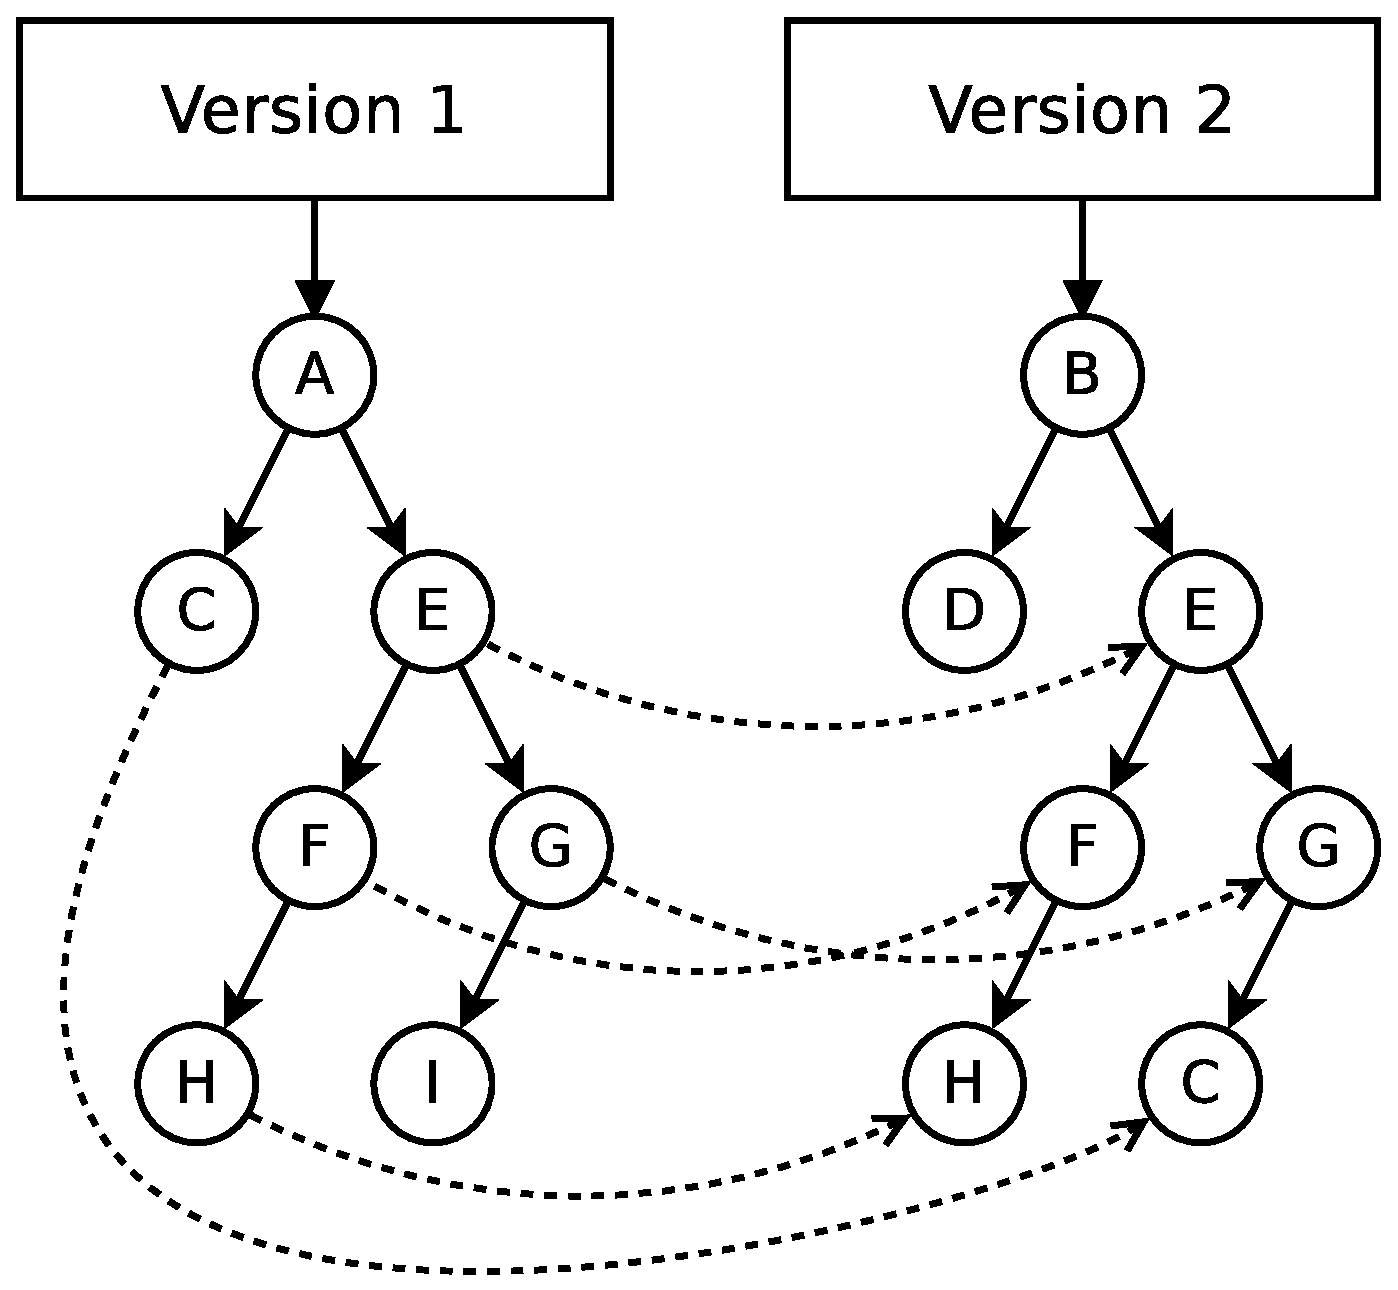
\includegraphics[width=0.65\textwidth]{figures/automatic_beh_inf/diagrams/dia2}
\par

\caption{Graphical representation of tree 
mapping\label{fig:tree-mapping-example}}
\end{figure}



\subsection{Cluster construction\label{sub:cluster-cons}}

Cluster construction comprises the grouping of nodes in subtrees,
and the readjustment of frontier links. Readjustment of frontier links is 
achieved
through the resizing of the clusters.


\subsubsection{Creating common subtrees}

At this point we have a mapping between the common nodes of both the
ASTs of the input modules. We now traverse the AST of one of the input
modules and we group in subtrees the pairs of contiguous nodes that
have a mapping. That is, we find those groups of mapped nodes that
are contiguous in both trees and the mapping.

We say that a pair of nodes $a$ and $b$ in a tree, (parent and child 
respectively),
are \emph{contiguous} if and only if: the parent of the projection of $b$
is identical to the projection of $a$, and $b$ is child of $a$
in the same position (numbering child nodes in order) as the projection
of $b$ as a child of the projection of $a$.

% In more formal terms, suppose that we are given two sets of nodes $N$ and $M$, 
(one per AST of
% input module, where $a,b\in N$), together with a function $f$ that maps pairs
% of common nodes from $N$ to $M$ ($f:N\rightarrow M$), (as returned
% by the tree matching algorithm in Section~\ref{sub:tree-matching}),
% and two functions $p$ and $q$, which map nodes in $N$ (and $M$ respecitvely) 
to their parents (together with their 
position among the children of that parent),
%  ($p:N\rightarrow(N,\mathbb{N})$ and
% $q:M\rightarrow(M,\mathbb{N})$). Then, two nodes $a$ and $b$ are said to be 
\emph{contiguous}
% if and only if: 
$\exists(i\in\text{\ensuremath{\mathbb{N}})}:(a,i)=p(b)\land(f(a),i)=q(f(b))$,
% or 
$\exists(i\in\text{\ensuremath{\mathbb{N}})}:(b,i)=p(b)\land(f(a),i)=q(f(b))$,
% or if there exists a node $c$ that is contiguous to both $a$ and
% $b$.

In Figure~\ref{fig:tree-clustering-example} we show how the trees
in Figure~\ref{fig:tree-mapping-example} would be clustered, where frontier 
links
are represented as dashed arrows.

\begin{figure}
\centering
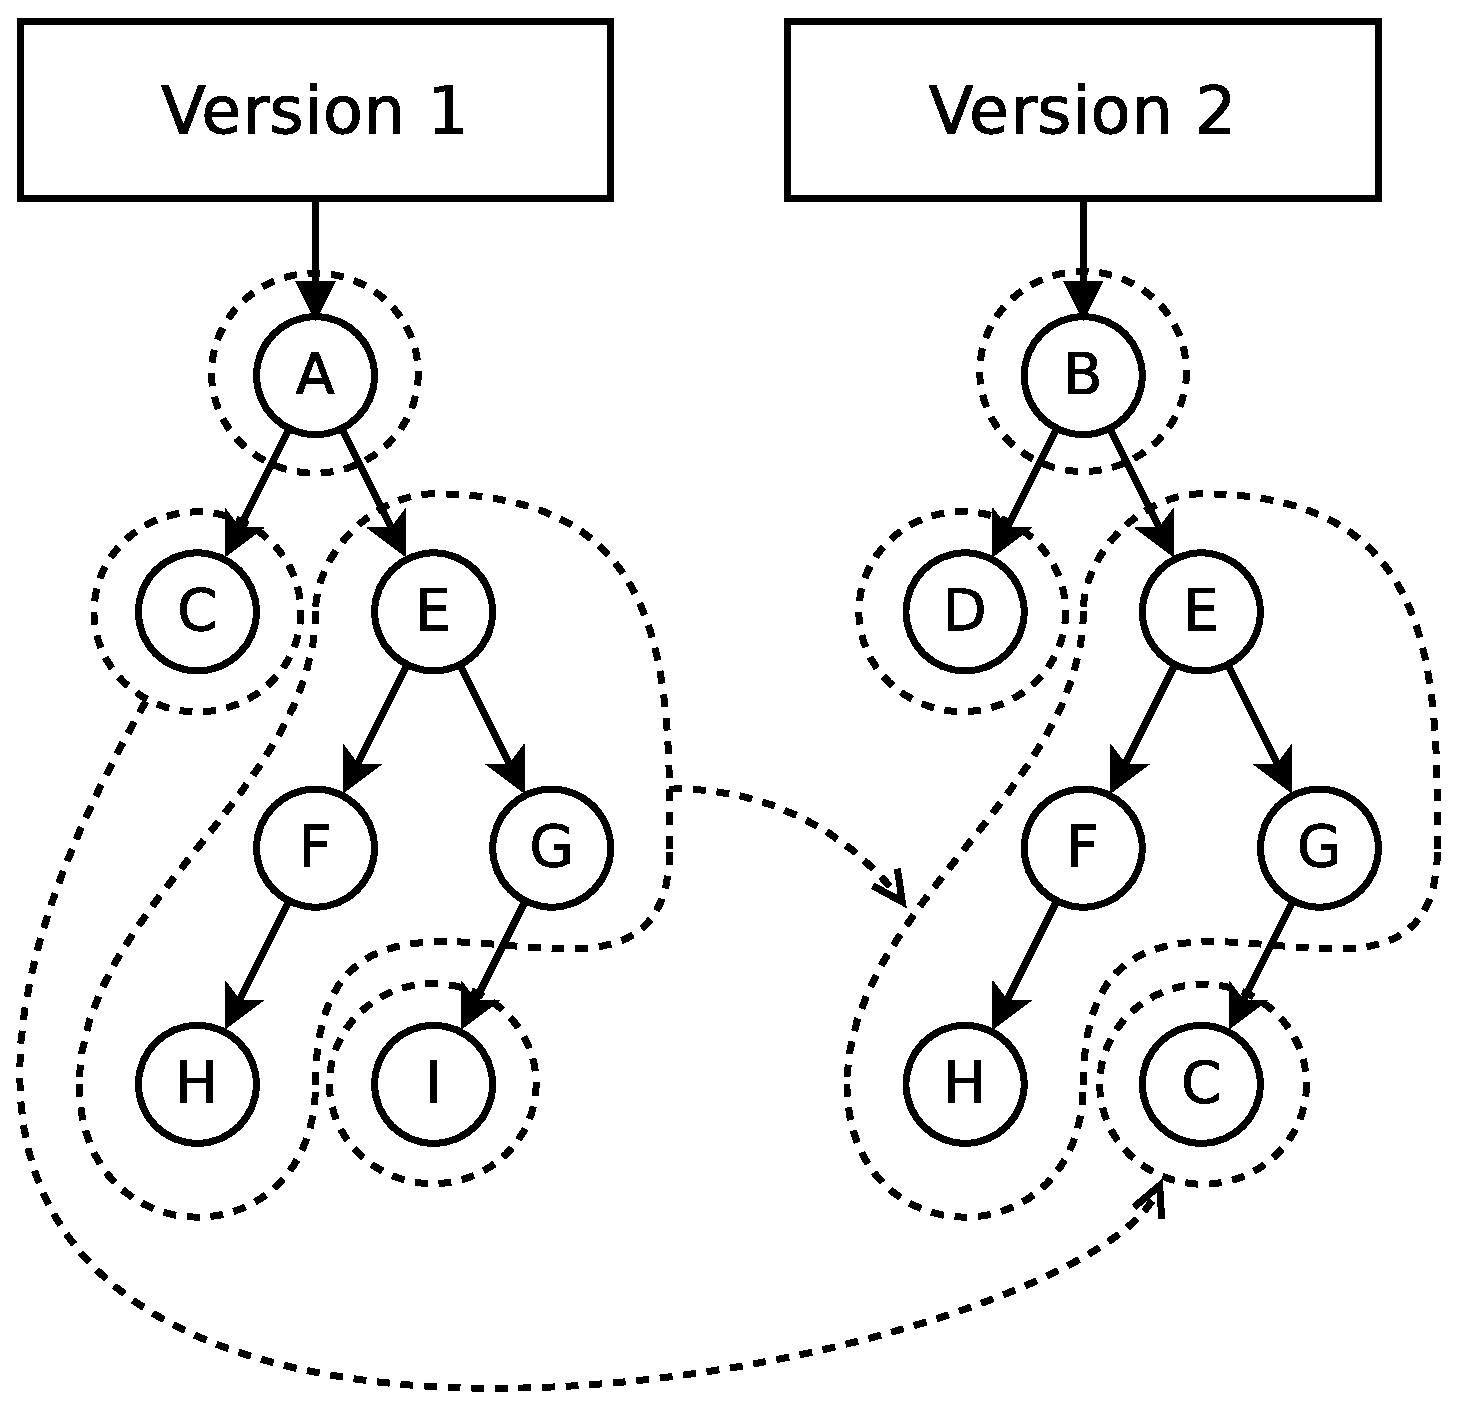
\includegraphics[width=0.69\textwidth]{figures/automatic_beh_inf/diagrams/dia3}
\par

\caption{Graphical representation of tree 
clustering\label{fig:tree-clustering-example}}
\end{figure}



\subsubsection{Readjusting the frontier links}

Once we have grouped all mappings in clusters, (i.e: contiguous subtrees),
we must check that the frontier links, (i.e: the pairs of parent-child
nodes with nodes in different clusters), are valid places for function
extraction. There are several reasons why this may not be the case,
the most common ones are:
\begin{itemize}
\item The lower node of the frontier link must be an expression. In particular,
it must be syntactically correct to use the subtree of the frontier link
as the body of a function.
\item It must be possible to replace the child node with a function call.
For example, a function call cannot be introduced in the header of
a function instead of a parameter.
\item The variables defined in the child subtree cannot be used outside
of it since creating a function will also create a new scope. This
can be allowed at this point and fixed afterwards in some cases.
\end{itemize}
The conditions for readjusting frontier links are also useful for fine
tuning the algorithm. We can allow the creation of invalid functions
as long as we have a post-processing mechanism that fixes them, (see
Section~\ref{sub:function-migration-artefact}), and we can disallow
the creation of functions that would be correct, if we want to preserve
some artefacts or for readability (see
Section~\ref{sub:artificial-block-expressions}).

We can adjust the frontier links by removing pairs of nodes from the common
clusters, and by removing their mappings. This produces a small replication
of code, but in the worst case scenario, we will fallback to having
no common clusters and that would leave the input modules as they
were originally.

We take as basic principle that, if necessary, we can have code common
to both instances replicated in both the behaviour instances, but
we cannot have code unique to one of the behaviour instances in
the behaviour definition. We could potentially do so by adding conditional
flow control expressions, but that would prevent future generalisation,
(the creation of new instances for the generated behaviour definition).


\subsubsection{Common clusters and unmatched clusters}

After we have computed the nodes that will form the clusters, we remove
them and their links from the ASTs, and we cluster for each ASTs
the groups of nodes that are still linked together into new ``unmatched 
clusters''.

We will now have two kinds of cluster:
\begin{itemize}
\item The common clusters, that have representation in both ASTs. Each of
them represents a function in the output behaviour definition (or
common functions).
\item The unmatched clusters, that in turn belong to one of the two ASTs.
Each of them represents a function in one of the behaviour instances
(or callbacks).
\end{itemize}

In Figure~\ref{fig:cluster-linking-example}, we show how the example
in Figure~\ref{fig:tree-clustering-example} would be reorganised
and linked, where the dashed node I in Version 2 is the rendering
of an indirection cluster.

Indirection clusters are unmatched clusters which have, as only body,
a function call that redirects the execution flow to the correct child cluster.

\begin{figure}
\centering
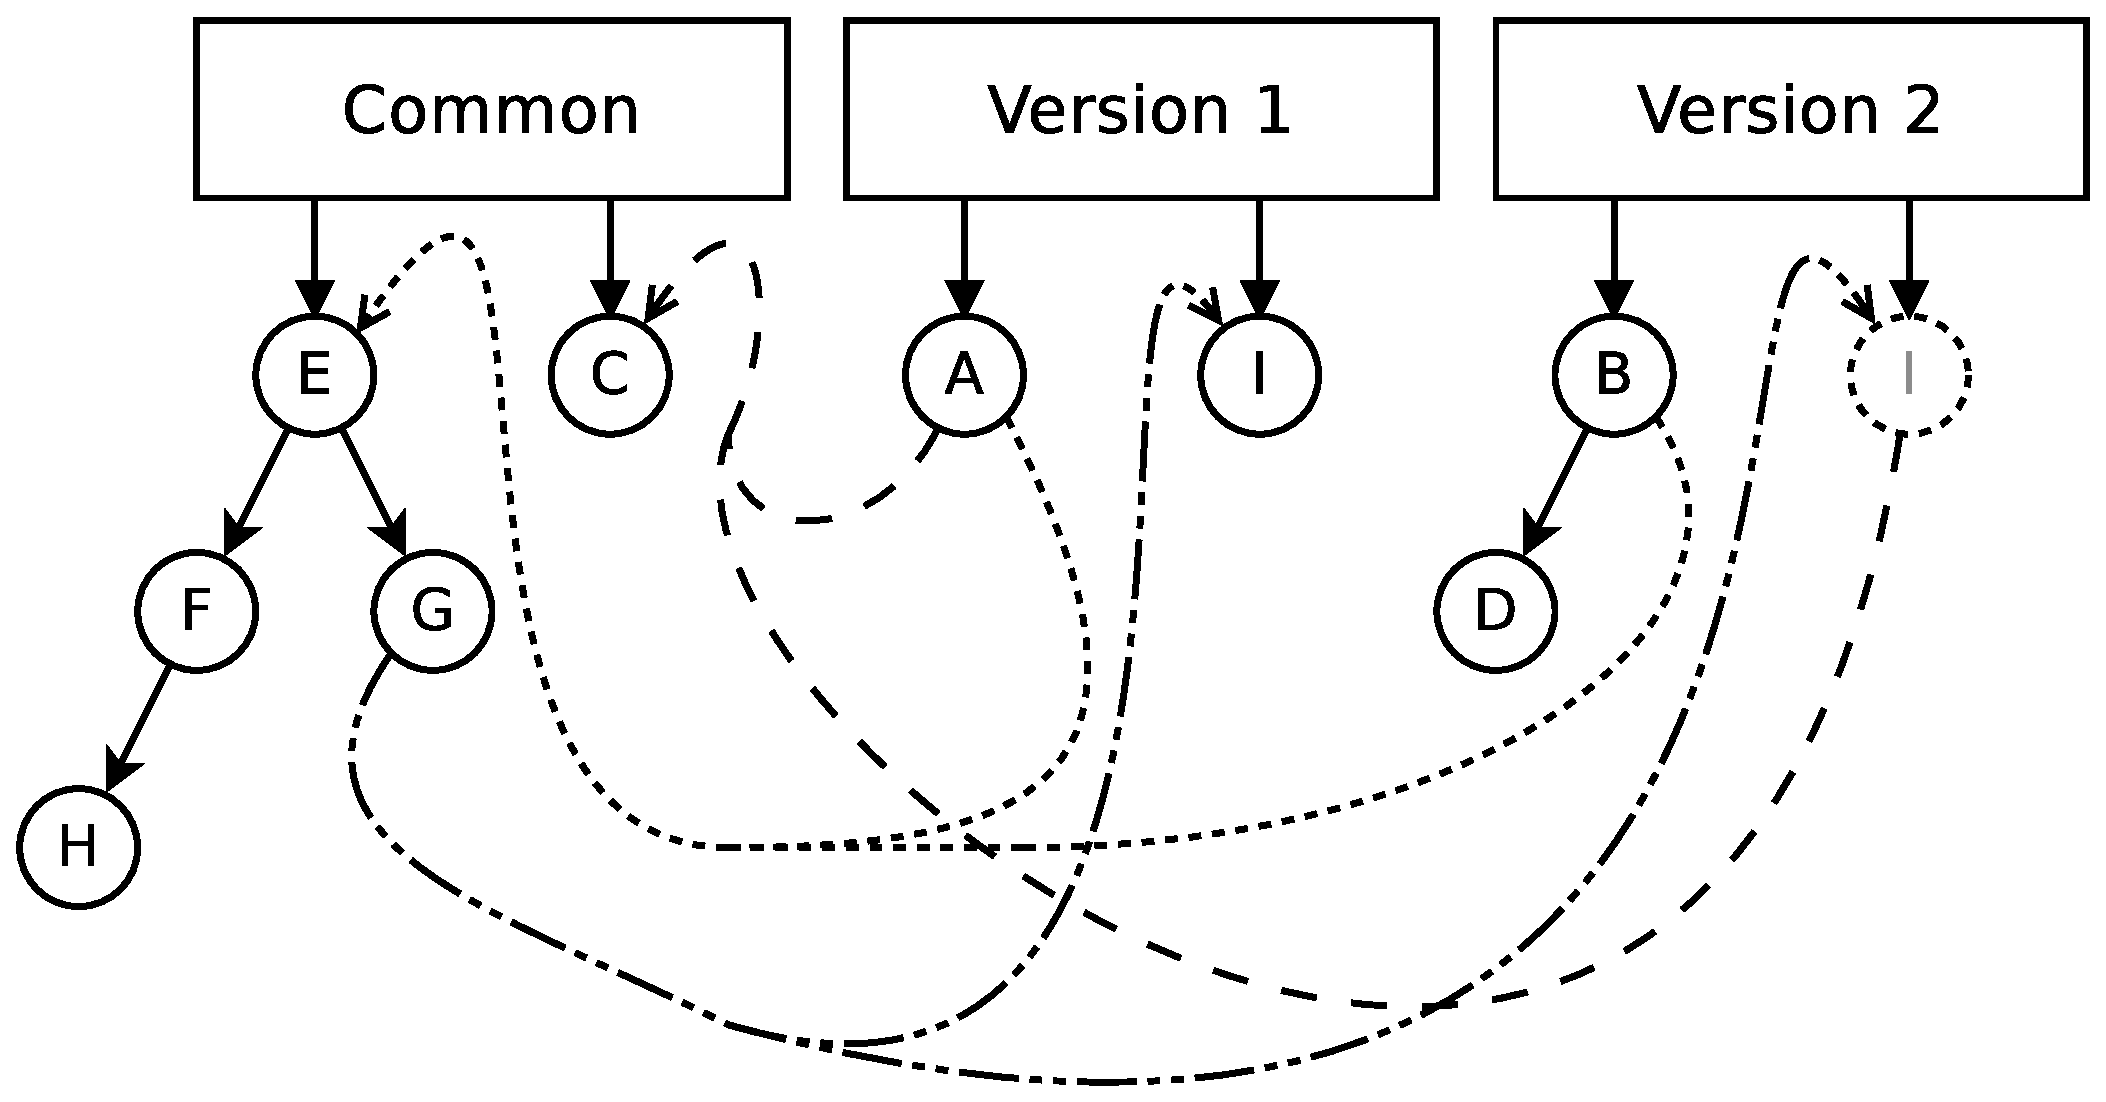
\includegraphics[width=1\textwidth]{figures/automatic_beh_inf/diagrams/dia5}
\par

\caption{Graphical representation of linking\label{fig:cluster-linking-example}}

\end{figure}

\subsection{Linking\label{sub:cluster-linking}}

The last step is linking the clusters through function calls, to preserve
the behaviour of the original modules after the relocation of the
functions.

For linking, we first visit every lower frontier link of common clusters,
and try to assign the same name to both alternative child clusters.
For each lower frontier link in the common clusters we necessarily have
two alternative child clusters, since nodes in the common clusters
are the result of merging two nodes. We also know that these two clusters
are different, since otherwise they would have merged to the parent
cluster. We can find which clusters these are by looking up the original
nodes in both of the original ASTs.

The alternative child clusters for a lower frontier link do not need to
be unmatched. It is possible that one or both of the child clusters
are also common. This is because the end of the cluster may be due
to a discontinuity in the mapping, rather than to unmatched code,

For example, a node $a$ and its parent $b$ may both have mappings and still
belong to different clusters if the image of $b$ is not the parent
of the image of $a$, or if the image of $a$ is in a different position
in the child list.

If that is the case, it is also possible that we have already set a
name for those clusters.

In order to create a uniform interface, we need to keep the symmetry
in both behaviour instances. This means having the same number of
callbacks in both instances, and having the same number of arguments
for each pair of equivalent callbacks.

Because of this, if we have already set a name for the cluster and,
thus, we cannot ensure that both child clusters have the same name,
we will create ``indirection clusters'' in either or both 
sides that cannot be renamed. Of course, we want
to minimise the use of indirection clusters, since they add complexity
to the code.

We can keep the number of parameters for equivalent callbacks equal,
by merging the parameter sequences of both alternatives at any point. If there
are common parameters, we add them only once, but we will add unmatched
parameters to both alternatives of each cluster. In the unmatched
side where the unmatched parameters of the opposite side are not bound,
we will use dummy values for those parameters. These dummy values
will not cause a difference in the behaviour because they will not
be used, and they are easy to generate thanks to the flexible typing
of Erlang.

\subsection{Extra considerations}

The automatic behaviour extraction refactoring subsumes several logical
sub-refactorings, and, thus, some considerations applied to these 
sub-refactorings
are also applicable to automatic behaviour extraction. The main logical
sub-refactorings implied by automatic behaviour extraction are: function
extraction, and function module migration, (i.e: moving one function
from one module to another).

But, of course, there are some considerations that are specific to
this refactoring as well.

\subsubsection{Artificial block 
expressions\label{sub:artificial-block-expressions}}

As we have mentioned before, when encapsulating code into functions,
we must ensure that the created functions are valid, and that it is
syntactically and grammatically correct to insert a function call
in the position where the extracted code originally was.

In addition, it is desirable that when several consecutive sentences
are extracted, they are combined into the same created function. This
is not trivial if, as in our implementation, the clusters created
have tree topology. Splitting a tree horizontally will create several
subtrees, which would in turn translate into separate functions. But
it is much clearer to have them grouped in the body of the same function,
rather than in several different functions which are called consecutively.
For instance, without the block artefact, the input example modules in 
Figure~\ref{fig:block-expression-input},
would be merged as shown in Figure~\ref{fig:block-expression-before},
the block artefact allows the more concise representation shown in
Figure~\ref{fig:block-expression-after}.

\begin{figure}
\begin{minipage}[t]{0.5\textwidth}%
\showcodehalfbox{figures/automatic_beh_inf/1-block_artefact/1-in/mod1.erl}
\end{minipage}%
\begin{minipage}[t]{0.5\textwidth}%
\showcodebox{figures/automatic_beh_inf/1-block_artefact/1-in/mod2.erl}
\end{minipage}

\caption{Input example modules to illustrate block expression 
artefact\label{fig:block-expression-input}}

\end{figure}

\begin{figure}
\begin{minipage}[t]{0.5\textwidth}%
\showcodehalfbox{
figures/automatic_beh_inf/1-block_artefact/2-out-before/mod1.erl}%
\end{minipage}%
\begin{minipage}[t]{0.5\textwidth}%
\showcodebox{figures/automatic_beh_inf/1-block_artefact/2-out-before/mod2.erl}%
\end{minipage}

\begin{minipage}[t]{1\textwidth}%
\showcodebox{figures/automatic_beh_inf/1-block_artefact/2-out-before/out.erl}%
\end{minipage}

\caption{Output of modules in Figure~\ref{fig:block-expression-input} without
block expression artefact\label{fig:block-expression-before}}
\end{figure}


\begin{figure}
\begin{minipage}[t]{0.5\textwidth}%
\showcodehalfbox{figures/automatic_beh_inf/1-block_artefact/3-out-after/mod1.erl
}%
\end{minipage}%
\begin{minipage}[t]{0.5\textwidth}%
\showcodebox{figures/automatic_beh_inf/1-block_artefact/3-out-after/mod2.erl}%
\end{minipage}

\begin{minipage}[t]{\textwidth}%
\showcodebox{figures/automatic_beh_inf/1-block_artefact/3-out-after/out.erl}%
\end{minipage}

\caption{Output of modules in Figure~\ref{fig:block-expression-input} with
block expression artefact\label{fig:block-expression-after}}
\end{figure}

\begin{figure*}
\begin{minipage}[t]{0.5\linewidth}%
\showcodehalfbox{figures/automatic_beh_inf/2-interference/1-in/mod1.erl}%
\end{minipage}%
\begin{minipage}[t]{0.5\linewidth}%
\showcodebox{figures/automatic_beh_inf/2-interference/1-in/mod2.erl}%
\end{minipage}
\vspace*{-2.5mm}
\caption{Input example modules to illustrate interference between 
artefacts\label{fig:interference-input}}
\end{figure*}



In our implementation we solve this problem by doing two passes to
the algorithm, after the first one, we locate the consecutive child
clusters and we introduce an artificial block expression around them
in both source modules. In the second pass, the blocks will be extracted
as a single function, and we can remove them easily at post-processing.
We also ensure that artificial blocks are not detached from their
child sentences by adding an exception for them in the frontier link 
readjustment
procedure.


\subsubsection{Exported variables}

Variables bound in a sentence of a function are accessible from the
following sequences of the function, even though they are located
at sibling subtrees. Because of that, if we extract part of a function
that defines variables used afterwards, we will move those variables
to a new scope, they will no longer accessible by the sibling trees,
and we will cause a compilation error.

For example, in the following function:

\begin{verbatim}
suma(A, B, C) ->
    Total = A + B,
    C = Total.
\end{verbatim}

We cannot directly move the first sentence to a different function
because the second sentence would not be able to access the variable
\texttt{Total}.

This problem can be prevented by ensuring, when adjusting the cluster
frontier links, that there are no variables exported to the parent cluster.
But when combined with the artificial block expression artefact, this
would be interfering, by preventing the extraction of bigger blocks
which could be fixed to preserve the semantics just by adding some
small artefacts, (see Section~\ref{sub:interference}).


\subsubsection{Exported variables in artificial block 
expressions\label{sub:interference}}

We can export variables from a function extracted as a block if we
make it return a tuple with the variables exported and we match them
outside of the function call.

But in some cases the result of the function may already be used from
outside, and modifying it would modify the behaviour of the refactored
program. To avoid this, whenever variables are exported, we will only
create artificial block expressions that do not contain the last expression
of a clause. We do not have to worry about modifying the value of
intermediate sentences in clauses, because we know that these values
were discarded in the original code. For example, in the code of 
Figure~\ref{fig:interference-input},
we cannot extract a common function for the whole clause of the \texttt{case}
expression because it both exports and returns values, but we can
create one function for the last expression and one for the rest as
shown in Figure~\ref{fig:interference-output}. This does not produce an ideal 
solution in every
case, and it is only implemented when the frontier link is in a clause,
but without it the previous approaches would modify behaviour in cases
where values are returned and exported simultaneously from a clause.

\begin{figure}
\begin{minipage}[t]{1\textwidth}%
\showcodebox{figures/automatic_beh_inf/2-interference/2-out/mod1.erl}%
\end{minipage}

\begin{minipage}[t]{1\textwidth}%
\showcodebox{figures/automatic_beh_inf/2-interference/2-out/mod2.erl}%
\end{minipage}

\begin{minipage}[t]{1\textwidth}%
\showcodebox{figures/automatic_beh_inf/2-interference/2-out/out.erl}%
\end{minipage}
\vspace*{-2.5mm}
\caption{Output of modules generated from those in 
Figure~\ref{fig:interference-input}\label{fig:interference-output}}
\end{figure}


In the second pass we will ensure that there are no exported variables,
(apart from those in artificial block expressions), to avoid breaking
other unusual kind of frontier links where we cannot automatically fix
the export of variables, (e.g: when the frontier link is between
the elements of a list and the list, and the element binds variables that
are used outside of the list). In those cases we will still keep the code
consistency in exchange for some replication by moving the frontier so that
it does not interfere with the variable scope.

\subsubsection{Module migration and dependencies}

Moving functions between modules also requires some considerations.
The behaviour of functions that must be moved may depend on the macros
used on the original module. Moving them without moving the macros
would alter their behaviour. These macros may define or import records,
external functions or macro definitions. In addition, these macros
may include conditionals, (i.e: \texttt{ifdef}, \texttt{ifndef}, \texttt{else},
and \texttt{endif}). There is no easy solution to combine the macros
of both modules that will work for every case. Because of this, we
opted for a compromise solution that will probably work for most cases,
we treat the outer conditional blocks of macros as single macros,
and we copy all the macros blocks that provide dependencies used in
the code that has been moved to the common module.

Another consideration to have when moving functions is to check that
none of the existing functions in the destination module conflicts
with the ones we are moving, in our case this is made easier by the
fact that the destination module is new and, as such, there are no
previous existing functions. Nevertheless, something similar can happen
for function whose name is not generated automatically (see 
Section~\ref{sub:function-arity-collision}).


\subsubsection{Function migration 
artefact\label{sub:function-migration-artefact}}
The headers of functions in Erlang, as in many languages, are hard to
divide through function extraction. Not being able to divide them
means that if two functions are very similar but they have slightly
different patterns, we are forced to keep the whole header of the
function in the unmatched modules and abstract only the body of each
of the clauses.

Nevertheless, if they are completely identical we can still generalise
them without modifying the interface. Even though we cannot insert
function calls on the root of a module, we can insert a very simplified
version of the interface of the function, move the whole function to the
common module, and insert a simple indirection.

We do this by accepting as a valid frontier link the division between the
header node of a function and the root nodes of the module, and by artificially
detaching, (i.e: removing from the mapping and common cluster), the
root node of the module.

During post-processing, we just have to generate the simplified function
header around the function call that is left in the place where the
original function was.


\subsubsection{Function arity collision\label{sub:function-arity-collision}}

Functions created in the common module may, at some point, need to
call the unmatched modules back. The right unmatched module to call
is the one that called the current function in the first place.

For Erlang to know which module to call we parametrise the destination
module of the function calls in the common module with a variable,
passed as a parameter by the calling module. This variable will contain
the name of the module as an atom at any particular time.

The solution is simple, but adding a parameter to common functions
will still modify its arity. This is not a problem when the names
of the functions are generated and each function has a different name.
But, because we only add the module parameter to those functions that
need it, if the function has been moved from the unmatched 
modules and has a name assigned by the user, it may potentially clash
with a different function which has the same name but different arity.

For example, we may have two functions with the same name, one with
three parameters, and other with four. If only the first function
requires us to add the module parameter, then we will end up with two
functions that have the same name and three parameters, which would
produce an error in compilation time.

It is necessary to have this in consideration, and rename one of the
clashing functions as soon as this happens, in order to avoid altering
the behaviour of the original code.

\subsection{Case study}
\label{sec:case-study}

We have successfully tried both techniques  (i.e. behaviour extraction and 
automated behaviour identification) in two QuickCheck models with two variants 
each:

\begin{enumerate}
 \item models for testing \texttt{ets} and \texttt{dets} term storage libraries, 
which are part 
of 
the Erlang standard distribution;
 \item models for testing the frequency server (extracted from 
\cite{CesariniThompson} and used as a case study in \cite{ExtractingQC}).
\end{enumerate}
These examples are included with the software deliverable and also 
included in Appendices~\ref{freq-server-code}~and~\ref{ets-dets-code}.

\subsubsection{Functionality}

Both techniques worked except for a small issue when applying the manual 
technique to a small piece of code that 
depended on a macro inside a conditional macro block. 

We now evaluate the results in more detail, examining some of the trade-offs 
involved in applying these techniques in practice as well as and 
possible alternatives and future improvements to the work.

\subsubsection{Parametrising the frequency server model}

For the frequency server model the automatic approach worked just as expected, 
since the difference was small and located in a single place. Parametrisation 
is done automatically in exchange for some automatically generated interface 
boilerplate code.

The manual approach for frequency server allows us to keep the 
interface of both modules common, but parametrisation of the 
unmatched part must be done manually, for example through a macro or by 
modifying the model manually.

\paragraph{Automatic approach.}

The frequency server example was simple, and the automatic approach 
already generated a good result by itself: we could see that the only 
unmatched method was the body of a precondition that in one was:

\begin{verbatim}
callback_1(Alloc, Freq) -> not lists:member(Freq,Alloc).
\end{verbatim}

and in the other:

\begin{verbatim}
callback_1(_Alloc, _Freq) -> false.
\end{verbatim}


For the automatic approach all the functions that existed in the input modules, 
which in this case had common body, were replaced in both instances with simple 
function calls that simply redirect the original interface to the common part, 
in order to keep the original behaviour unchanged.

This is good because we would not have to modify any module that uses the code 
generalised, it all works the same as it did. In exchange we have a small 
amount of boilerplate that clutters the code.

\paragraph{Manual approach.}

For the manual approach we just need to select the body of the function that 
changes. We already knew which part it is thanks to the automatic approach, 
but we could have found out with a tool like \texttt{vimdiff}, for example.

We select the piece of code that changes in one of the input instances, and 
apply the refactoring \texttt{Expression to behaviour instance} pointing to a 
new nonexistent module. The new module will contain the unmatched code for that 
version.

We can now copy the instance we generated and modify the callbacks to contain 
the code corresponding to the other version. In this case, if we selected the 
most complex version, we just have to replace the code of the callback with the 
atom \texttt{false}.

As described in Section~\ref{sub:alternative-adjustments-for-generalisation} we 
must also generalise the calls to the \emph{behaviour instance} callbacks. In 
our case study we replaced them with a macro that we called 
\texttt{?BEH\_INSTANCE}.

\subsubsection{Parametrising the ETS and DETS models}

For the \texttt{ets} and \texttt{dets} models the automatic approach produces 
correct 
results but the number of callbacks and common functions generated is 
high. Some preliminary clone removal reduces the amount of functions 
generated but it is still higher.


The manual approach allows for more meaningful divisions, but we found 
very useful to get assistance from a diff tool like \texttt{vimdiff}. Again we 
can have a shared interface but we need to parametrise the model 
manually.

\paragraph{Automatic approach.}

The models for \texttt{ets} and \texttt{dets} were more difficult to 
parametrise. For the ETS and DETS models, the automatic approach abstracts an 
important part of the code automatically, and the result, one more time, 
preserves the behaviour of the original code. But on the first attempt, the 
result of applying the automatic approach made it obvious that some prior clone 
removal was necessary in order to avoid the creation of several identical 
callbacks:

Several of the extracted functions contained the same body, (in particular the 
atoms \texttt{ets} and \texttt{dets} in both instances respectively). The 
reason 
is that automatic behaviour extraction does not remove clones it only matches 
the code of one input module with the other.

We used this cue to remove the replication and generalise the atoms into 
separate functions in the original modules. We used for this the refactorings 
\texttt{Function extraction} and \texttt{Fold expression against function}.

In particular we extracted two functions \texttt{module\_name/0} with 
the name of the API module (\texttt{ets} and \texttt{dets} atoms respectively), 
and \texttt{table\_name/0} with the name of the test table (\texttt{ets\_table} 
and \texttt{dets\_table} atoms respectively)

With this generalisation we reduced the number of common functions to 23 and 
the number of callbacks to 40.

Even after clone removal some of the callbacks generated by the automatic 
approach -- despite being correct -- may arguably be hard to understand for 
humans, specially because generated callbacks do not have meaningful names. For 
example, the code in Figure~\ref{fig:auto-abs} would hardly be abstracted out 
by 
a human because it does not have a meaning, but it is indeed common to both 
instances and it is technically correct to abstract it out.

\paragraph{Manual approach.}

For the manual approach we used as starting point the modules with functions 
\texttt{module\_name/0} and \texttt{table\_name/0} created for the automatic 
approach, and we were more conservative. For example, whenever several 
sentences 
or clauses changed within the same function, we considered parametrising the 
whole function instead of several of its parts.

To find out which parts of the modules to extract when using the manual 
approach we used \texttt{vimdiff} to understand the differences. We used one of 
the instances to iteratively extract the unmatched parts, and then we made a 
copy of the generated \emph{behaviour instance} and replaced the bodies of the 
functions with the equivalent bodies of the other instance.

Finally we generalised all the calls to the \emph{behaviour instance} by 
replacing the module name with a macro called \texttt{?BEH\_INSTANCE}.

Additionally, we had to manually add the functions that were in one of the 
instances but not in the one that we used as starting point.

With this procedure we generalised the implementation by introducing only 11 
callbacks and no common functions, but we introduced a small amount of 
replication too.

The only issue we found is that the manual refactoring crashed when trying to 
move a function that contained a macro that was defined inside a conditional 
macro block.

\begin{figure}[t]
\showcodeboxwithlabel{lst:auto-abs}{figures/automatic_beh_inf/auto_abs.erl}%
\vspace*{-2.5mm}
\caption{Behaviour definition and instance after extraction\label{fig:auto-abs}}
\end{figure}

\subsubsection{Future work}

Results suggest that future work could improve our automatic approach by 
allowing the manual refining of matched and unmatched parts through an 
interactive interface. The same could be applied to the manual approach.

Automatic parametrisation could be applied to the manual approach, but that 
would require a more global approach instead of an iterative one.

\section{EFSM Inference}
\label{EFSMInference}

\subsection{EFSM Semantics}
\label{EFSMSemantics}

Extended Finite State Machines extend conventional Finite State Machines by incorporating a \emph{data state} in addition to the \emph{control flow} state of the standard machine. This data state is described in \cite{EFSMs} as an n-dimensional space that can store values. The transition labels are extended to incorporate \emph{guards} (called \emph{enabling functions} in \cite{EFSMs}) that are boolean functions over the data space. The available transitions of the machine depend not only on its control flow state (as is the case for FSMs) but also on its data state, as some transitions may be prevented by their guards. Additionally, EFSM transition labels contain \emph{update} transformations that modify the data state if the transition is executed. 

The model of EFSMs used in this paper extends on that from \cite{EFSMs}, where the guard and update transitions operated solely on the data state. The model used here makes the guard and update transitions functions over both the data state and the inputs. This allows the machine to express guards on parameterised, named events, and to incorporate input parameters into its data state.
  
An EFSM is formally defined as an 9-tuple $M = (S,L,I,O,D,G,U,F,T)$ where:

\begin{itemize}
\item{$S$ is a set of symbolic states}
\item{$L$ is an alphabet of event labels}
\item{$I$ is a vector space of inputs, $i_{1} .. i_{n_i}$}
\item{$O$ is a vector space of outputs, $o_{1} .. o_{n_o}$}
\item{$D$ is a vector space $r_{1} .. r_{n_r}$ that represents the internal \emph{data state} as a series of registers}
\item{$G$ is a set of boolean guard functions $g_{i} : (I \times D) \fun \bool$}
\item{$U$ is a set of update functions that compute a new data state from the inputs and the previous data state $u_{n_u} : (I \times D) \fun D$}
\item{$F$ is a set of output computation functions that produce the outputs from the data state and input parameters $f_{n_f} : (I \times D) \fun O$}
\item{$T$ is a transition matrix $T : (S \times S) \fun \powerset (L \times G \times U \times F)$}
\end{itemize}

This structure is very similar to the \emph{Stream X-Machine} presented in \cite{StreamXMachines}, only it does not model the \emph{streams} of inputs and outputs, instead treating them as instantaneous, external actions.

EFSMs are presented throughout this document as graphs, with the nodes representing the symbolic (or control flow) states from the set $S$, and the transitions labeled with representations of the label, guard, output, and update functions for that transition. These are presented as a label, a comma separated list of guard functions in square brackets followed by a slash, and then a list of output functions, and finally the update functions in square brackets. The list of guard functions is logically conjoined, but is often more readable as a list rather than a single large expression, and there are implementation advantages to being able to apply list concatenation operations. The output and update functions must all assign different elements of the respective spaces, but they operate over the anterior state only, so they can be considered to occur concurrently.

The update and output functions use the assignment syntax $:=$ to identify the value in the vector space that is computed. Any data state variables not computed explicitly are defined to be unchanged from their value before the transition; any input or output values that are not computed are assumed to be undefined (i.e. that input parameter is not present or that output value is not produced in this transition). Outputs and updates are represented using the same syntax. Outputs are presented immediately after the slash ($/$), while updates are inside square brackets. All output and update expressions operate over the anterior state of the data registers, so $f[r_1 = 7]/o_1 := r_1 [r_1 := r_1 + 1]$ will result in $o_1$ being assigned the value 7, and the posterior state of $r_1$ will be 8.

The general form of a transition is: 

\begin{center}
$s_n \xrightarrow{e[g_1, .. g_{n_g}]/o_1, .. o_{n_o} [u_1, .. u_{n_u}]} s_m$ 
\end{center}

The arrow above represents a transition from state $S_n$ to $S_m$ with the event label $e$, restricted by guard expressions $g_1$ through $g_{n_g}$, producing outputs defined by $o_1$ through $o_{n_o}$, and updating the data state according to $u_1$ through $u_{n_u}$. The guard expressions are logically conjoined --- i.e. they must all be true for the transition to be allowed. Similarly, the output and update expressions should not be contradictory. In practice there will be one output or update expression for each output produced and each data state register that is altered. For example:

\begin{center}
$s_n \xrightarrow{vend[r_{2} \geq 100]/o_{1} :=r_{1}[r_{2} := r_{2} - 100]} s_m$
\end{center}

This arrow represents a transition that occurs with the event $vend$ when $r_2$ is greater than 100, and produces the output with a value from the data space variable $r_1$, and updates the data space variable $r_2$ by subtracting 100 from the previous value. If there are no guard expressions or no outputs or updates then the relevant section can be omitted entirely:

\begin{center}
$s_1 \xrightarrow{select[i_{1}="coke"]} s_2$

$s_4 \xrightarrow{vend/o_{1} := r_{1}} s_5$
\end{center}

A simple EFSM model of a vending machine is shown in \fig{fig:vendsimple}. This shows a machine which begins with a $select$ operation that stores its input values ($i_1$ - the chosen drink) in data state register $r_1$. Then it allows $coin$ operations and increases the value of $r_2$ by the value of $i_1$ (the value of the inserted coin). A $vend$ operation is prevented by a guard expression until the value of $r_2$ reaches or exceeds 100. At this point a $vend$ operation can be performed which will decrease $r_2$ by 100 and output the selected product (stored in $r_1$).

\begin{figure}[h]
\begin{center}
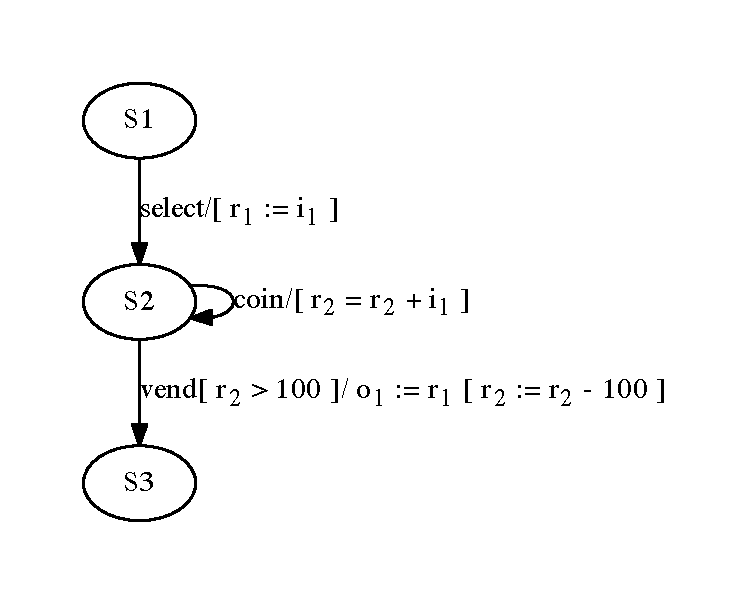
\includegraphics[width=7cm]{figures/efsm/vend-real.pdf}
\caption{A simple vending machine EFSM}
\label{fig:vendsimple}
\end{center}
\end{figure}

This model doesn't define any limits on the chosen products, nor does it allow the user to continue after the $vend$ operation. A more complicated model of a vending machine that keeps track of stock levels for two products and gives change is shown in \fig{fig:vendcomplicated}.

\begin{figure}[h]
\begin{center}
\hspace*{-1.5cm}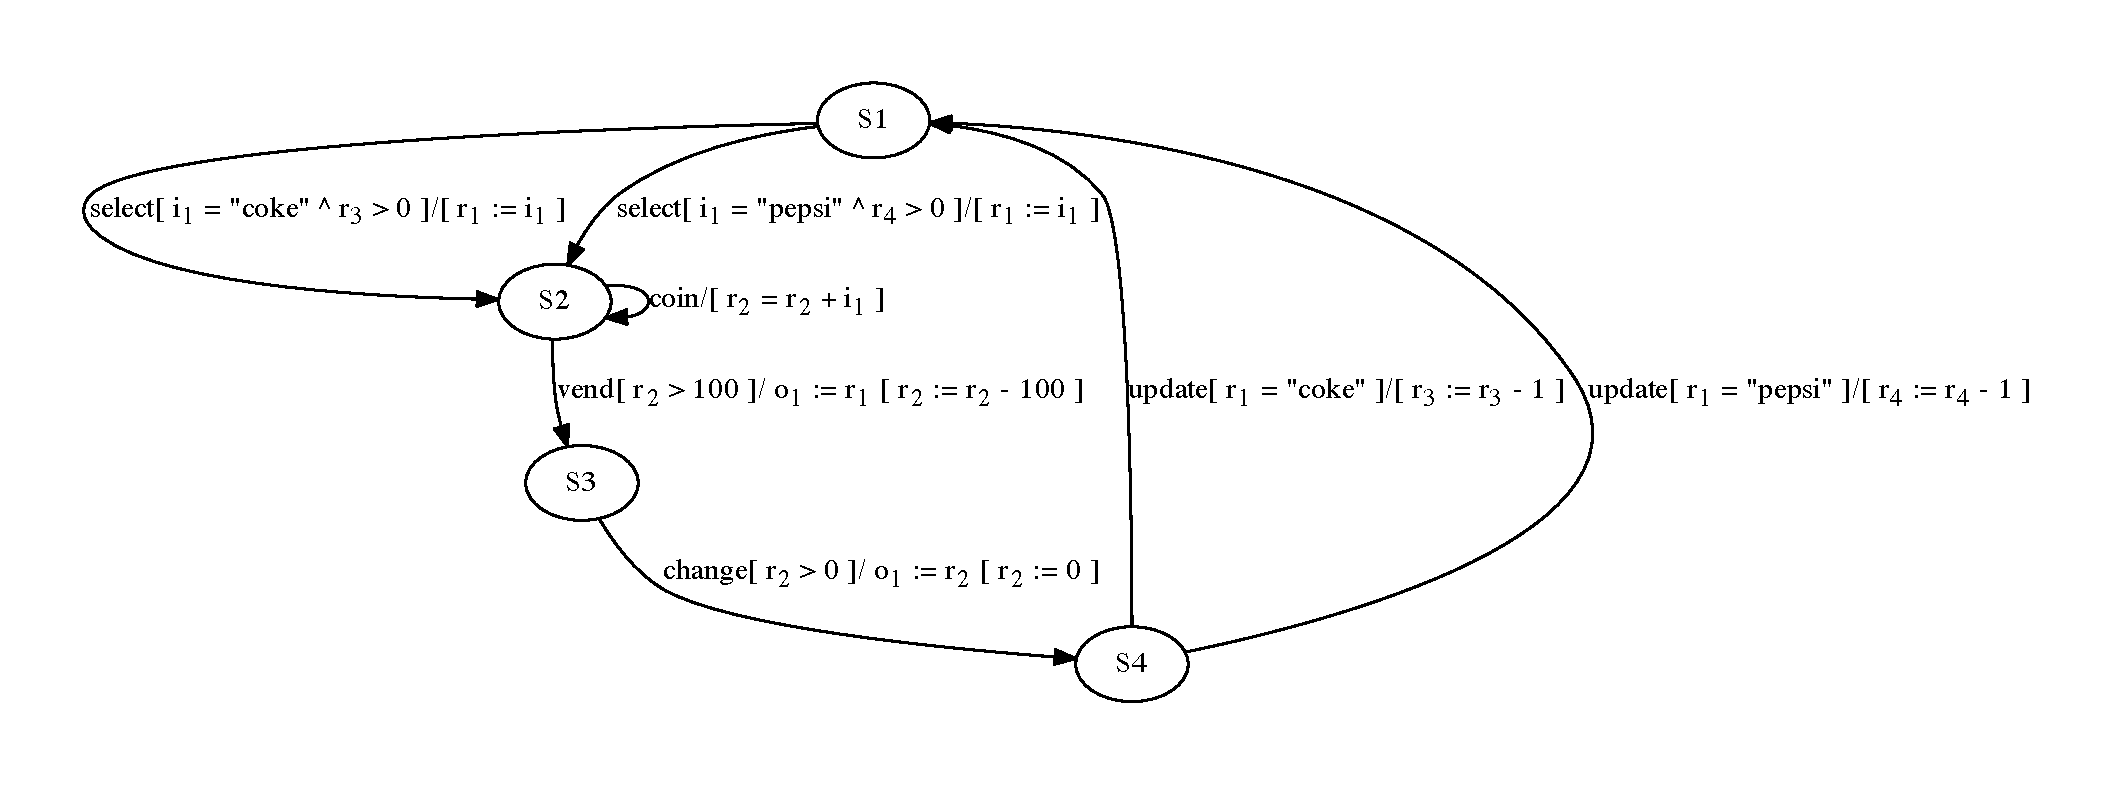
\includegraphics[width=18cm]{figures/efsm/vend-complicated.pdf}
\caption{A more complicated machine EFSM}
\label{fig:vendcomplicated}
\end{center}
\end{figure}

\subsection{Guard and Update Expressions}
\label{Expressions}

The EFSM guard, update, and output expressions make use of various operators. Guard expressions use conventional comparison operators ($<, \leq, >, \geq$) and equality symbols ($=, \neq$) and have boolean values.

Update and output expressions use an assignment syntax of the form $o_n := <expression>$, where the expression has some appropriate value. Conventional arithmetic is supported ($+,-,*,/$), and literal values are enclosed in quotes (e.g. $"coke"$). Literals that are numeric are assumed to be converted automatically, so $o_1 := r_1 + "12"$ is valid. 

As well as the conventional comparison and arithmetic operators, this work introduces operators for string comparison and extraction. In many protocols the values that must be stored in the internal data state are not present in isolation, but as parts of larger blocks (network data packets, for example). The inference process described in \sect{Algorithm} is designed to operate without prior knowledge of the structure of the data. 

Consequently, the operators $match(pre,suf,var)$ and $get(pre,suf,var)$ are introduced to express the existence of values within strings, and to extract those values. They are designed to identify and extract vales by reference to prefix and suffix strings in the protocol. These can be the empty string, if the required value is consistently at the beginning or end of the string, or is the entirety of the string. 

The $match$ operator can test whether a string matches a general pattern --- containing a variable value surrounded by a specific prefix and suffix, but not necessarily at a given position\footnote{This was designed to support HTTP style key-value pairings, where the order of pairings is not enforced but their syntax makes them identifiable.}. The $get$ operator is used in output and update computations and retrieves the variable value from such a pattern. For example, in the event that $i_1 = "key=xyz;"$ the expression $match("key=",";",r_1)$ would evaluate to $true$ (since the value of $r_1$ does contain a variable component that is prefixed by $"key="$ and suffixed by $";"$), while the expression $get("key=",";",r_1)$ would evaluate to the string $"xyz"$. The application of these operators is still experimental and is not applied extensively in the examples. The expressions $match("","",x)$ and $get("","",x)$ are equivalent to $true$ and $x$ respectively.

\subsection{Inference algorithm}
\label{Algorithm}

This section describes the process of inferring Extended Finite State Machines from parameterised traces in a way that builds on previous PROWESS work to infer Finite State Machines \cite{d31,d32}. It also introduces the open-source Athena \cite{Athena} EFSM inference implementation that was developed in this work package.

The inference process follows a similar pattern to the FSM inference processes, in that it begins by forming the observed traces into a Prefix Tree Automaton, and then merges states in the PTA where heuristics imply that they are likely to be separate instances of a single, more general behaviour. In addition to merging the \emph{control flow} states, the Athena EFSM inference implementation also merges and generalises the transitions. Where the conventional state merging heuristics merge two states this can produce situations where multiple transitions with the same label connect the same pairs of states. Taking the merging of the states as evidence that the two transitions are instances of a single system behaviour, Athena will generalise the guards, output computations, and data state update functions to represent all the observed instances. This generalisation combines well with an iterative approach to learning, since generalisations over early traces can often incorporate later instances of the same behaviour --- when those traces are added to the EFSM model they will simply walk over the existing, general transitions without adding new transitions or states that need merging\footnote{Their trace and event number details are added to the relevant transitions' logs, though, in case there is a contradiction detected later.}.

In addition to generalising transitions at particular points in the state machine, the Athena implementation also analyses the observed data values and generalises over patterns of data re-use. EFSMs extend on FSMs by allowing data to be retained in the data state of the system. The purpose of this data retention is to either use the data for comparisons, or for computations at a later point in the system's execution. Some previous work on parameterised state machine inference has modelled this by simply retaining all data in the system state, but the Athena implementation identifies specific instances where data re-use is observable in the traces, and then generalises over patterns of this re-use in multiple traces, in the same way that the state merging heuristics identify repeated patterns of events to indicate likely equivalent behaviour. This allows the Athena implementation to grow the data state systematically, incorporating new data registers only when there is an evidence-based reason for doing so.

The following subsections describe each stage of the inference process in more detail.

\subsubsection{Prefix Tree Automaton generation}
\label{PTA}

As with previous FSM inference algorithms \cite{BlueFringe,QSM,NeilQSM,StateChum}, the EFSM inference process begins by producing a Prefix Tree Automaton (PTA) from the traces. Since EFSM models incorporate data, the trace events are parameterised with each event potentially including several arguments and outputs. To form the PTA --- which is an EFSM itself --- these trace elements must be converted to EFSM transitions. To do this the events are converted into the very specific transitions that include guards that require exactly the arguments presented, and output computation functions that simply produce the literal value observed.

\begin{figure}[h]
\begin{center}
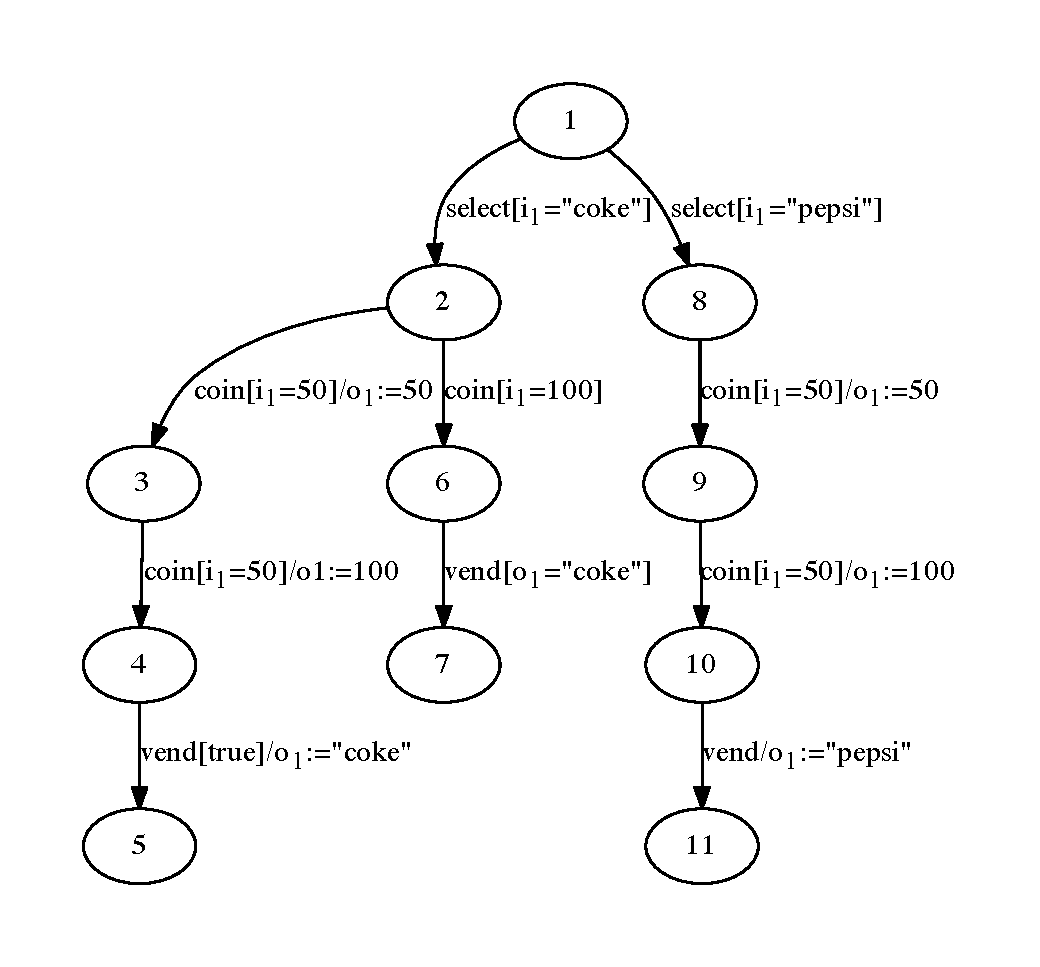
\includegraphics[width=12cm]{figures/efsm/vend1.pdf}
\caption{The Prefix Tree Automaton (PTA) of the vending machine}
\label{fig:pta}
\end{center}
\end{figure}

An example of a PTA produced from three traces is shown in \fig{fig:pta}. However, the addition of data to the transitions means that comparing states and transitions in EFSMs produces an extremely high complexity. To counter this, the Athena implementation operates an iterative process. The initial PTA is build from the first two traces and the subsequent traces are added one-by-one later. This allows the generalisation stages described in the following sections to operate on reasonable numbers of states and transitions and allows the complexity of the comparisons to be practically applied. This process of early generalisation can be very effective, since later traces --- by definition --- instances of the general rules of the program they can often be added trivially to an EFSM model that has already inferred the general rules from early traces.

Adding a trace to an existing EFSM is a simple process of walking through the EFSM and following transitions that match both the event label and data constraints of the trace. Once a point is reached at which no transition matches the next event a new transition can be added to a new state. From here, the remainder of the trace is added as specific transitions to further new states. 

This can produce non-deterministic EFSMs if the newly added transition conflicts with an incorrect generalisation that has been inferred from the previous traces. This is then resolved by the \emph{splitting} process described in \sect{Splitting}.

That the traces are added iteratively can mean that particular orderings of the traces will cause the model to resolve more quickly than others, but the process of merging and then splitting on contradictions, and then re-merging continues until the model reaches a stable state such that further merges are scored below some user-defined threshold. This results in a consistent eventual model regardless or trace order. As well as reducing the complexity of any one iteration of the algorithm, the iterative approach allows the Athena implementation to operate over \emph{live} data, stabilising its model based on what it has observed \emph{so far}. With this as a design intention there has not been any emphasis placed on identifying particularly good or bad orderings, since this would not be controllable in a live learning scenario. 

\subsubsection{Evidence Driven State Merging}
\label{EDSM}

The current Athena EFSM inference implementation uses an extension of the K-Tails algorithm \cite{KTails}. This compares every pairing of control flow states and measures the similarity of their \emph{tails} --- that is the reachable sequences of events to some length \emph{k} from each state. For EFSMs this comparison has to be extended to consider the similarity of the data components: guards, output computations, etc. 

Guard expressions are compared both for logical similarity --- equivalence, implication, or subsection --- and their data dependences, so $r_1 = 3$ and $r_1 = 4$ are more similar than $r_1 = 3$ and $i_3 = "fish"$. This is significant, since logically distinct guards, such as $r_1 = 3$ and $r_1 = 4$, that refer to the same variables may be specific instances of a more general rule --- e.g. $r_1 < 5$.

A similar approach is applied to output computations and update functions, scoring highly for instances where one function is a specific instance of the other, more general function --- e.g. $o_1 := 7$ and $o_1 := r_1 + 1$.

This produces a triangular matrix of \emph{scores} for pairings of states. The highest scoring pair will be the first candidate for merging. The algorithm proceeds by forming a new state and modifying all transitions that terminated with either of the original states to terminate with the new state, and all transitions that originated from either of the original states now originating from this new state.

This can identify compatible transitions if the newly merged state causes some transitions with identical labels to have matching origin and destination states. Alternatively, it can produce a non-deterministic EFSM if several transitions have the same label, different destinations, and overlapping guards. Both of these instances are handled by the generalisation process.

\begin{figure}[h]
\begin{center}
\begin{minipage}{0.45\textwidth}
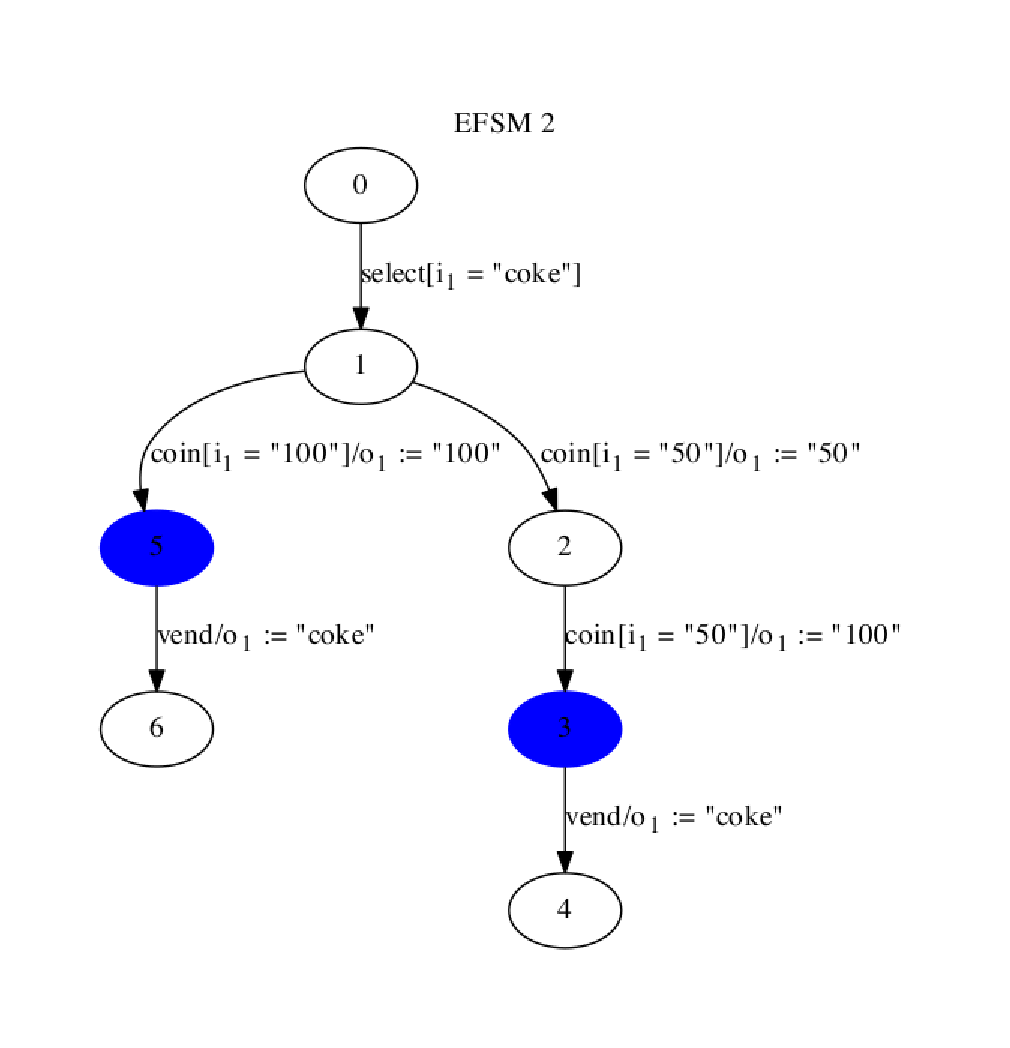
\includegraphics[width=8cm]{figures/efsm/premerge.eps}
\caption{A PTA built from the first two traces of the vending machine, with selected merge states highlighted}
\label{fig:premerge}
\end{minipage}
\begin{minipage}{0.45\textwidth}
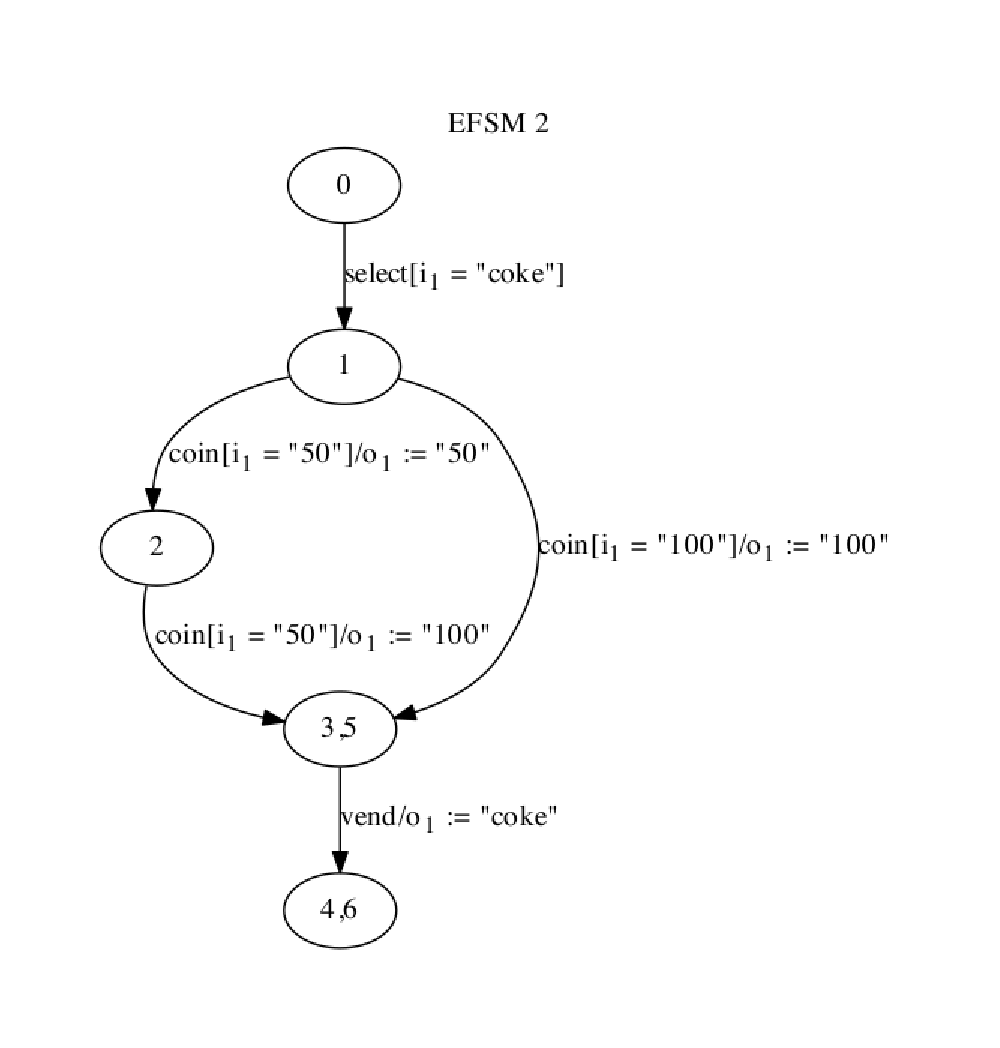
\includegraphics[width=8cm]{figures/efsm/merge1.eps}
\caption{A merge from the first two traces of the vending machine}
\label{fig:merge}
\end{minipage}
\end{center}
\end{figure}

\fig{fig:premerge} shows the result of building a PTA from the first and identifies states 5 and 3 as the best merge, due to their identical (if short) tails. \fig{fig:merge} shows the result of merging states 3 and 5, as selected by the EDSM scoring from \fig{fig:premerge}. This resulted in states 4 and 6 being merged as well, due to the identical transitions 

\subsubsection{Generalisation of transitions}
\label{Generalisation}

Where state merging produces sets of transitions with identical labels, and origin and destination states it is likely that these are different instances of the same behaviour. In this case the inference process produces a single transition that generalises all the observed instances.

To merge distinct guard expressions, the Athena implementation uses an approach based on Inductive Logic Programming \cite{ILP}. All boolean expressions in the simple guard expression language can be placed in a lattice, and the most specific generalisation of a set of guard expressions is their least upper bound. In the Athena implementation, this is more general than a simple disjunction, but it is a deliberate overgeneralisation. Strictly, the least upper bound of $i_1 = 3$ and $i_1 = 4$ is $(i_1 = 3) \lor (i_1 = 4)$, but simply using the disjunction of observed instances would produce unwieldy guard expressions and would not provide any way to predict the outcome of unobserved instances (the trace where $i_1 = 2$, for example) so the Athena implementation will choose a more general expression such as $i_1 < 5$ or $i_1 > 2$ depending on whether there are any alternatives with the same label and different destination states. State machine inference approaches always operate by overgeneralising to allow predictions. Over-generalisations that are contradicted by traces observed later are discussed in \sect{Splitting}.

Where the merged transitions have different destinations will cause the Athena implementation to immediately attempt to merge the targets. A process of \emph{zipping} occurs as a state merge causes a chain of states to be merged with each other --- such as the merging of states 4 and 6 in \fig{fig:merge}. This is a common occurrence where several branches of the PTA are really instances of the same behaviour and merging of their first element identifies this. In the event that a later element of the branches contradicts, this zipping can be undone --- either in part or in full --- by the contradiction resolution procedure described in \sect{Splitting}.

Merging of output and update computation functions cannot be done by simple generalisation, since it must remain computable --- the EFSM models produced by the Athena implementation are intended to allow simulation as well as classification, so they must be able to produce the outputs and new data state as well as confirm that they are acceptable. However, due to the simple nature of the expression language it has been found that Genetic Programming \cite{GeneticProgramming} can be used effectively. The generic programming approach used in the Athena implementation begins with a population of randomly generated expressions over the input and register spaces and measures how many of the observed instances are correctly predicted by each member of the population. Those that predict the largest percentage of instances are retained and are both \emph{bred} and \emph{mutated} for subsequent rounds. 

The \emph{breeding} of two expressions operates on the abstract syntax tree of each expression, and cuts each tree at a random node. The sub-tree of one expression is then grafted onto this node of the other tree to form a new expressions. For example, $o_1 := i_1$ and $o_1 := i_2 - r_1$ might be bred to form $o_1 := i_1 - r_1$. This approach is particularly effective because it is often the case that a moderately accurate expression is referencing some of the correct parts of the state but not all, so the combinations can improve this.

Additionally, \emph{mutation} of expressions occurs by changing one element of the parent expression --- this includes operators, variable names, and literal values. New literal values are not chosen completely at random, since that would produce large numbers of spurious results, but are instead chosen from within the range of values observed plus/minus a small delta --- so, if values 2,3, and 5 had been observed the implementation may choose 4 or 1 as a fresh literal, but would not choose 4,096. A mutation operator that has proven particularly effective is the \emph{nudge} operator, which modifies a literal by a small delta. This is particularly effective where there are comparison operators and the previous generation of expressions was classifying many but not all observed values correctly --- $i_1 < 56$ when the true guard expression is $i_1 < 50$, for example, achieves a high accuracy when the samples include 45, 54, 58, and 65, but a small nudge creates a correct expression.

The genetic programming is time-budgeted, so the implementation will not wait indefinitely for an answer, but it was able to produce appropriate results for a range of test cases when limited to 100 seconds with a population size of 40. Where no suitable resolution can be found the state may need to be split, so the EFSM model is passed on to the contradiction resolution procedure described in \sect{Splitting}.

\subsubsection{Identifying co-incidence of data re-use}
\label{IntertraceDependencies}

Both the ILP based generalisation, and the Genetic Programming are only able to generalise expressions over the data state that is represented. When the PTA is initially created there is no information about the internal data state of the system. Rather than include excessive information in the data state --- particularly as this would widen the search space for genetic programming --- the Athena inference implementation only adds a register to the model if it observes evidence of data re-use.

\begin{figure}[h]
\begin{center}
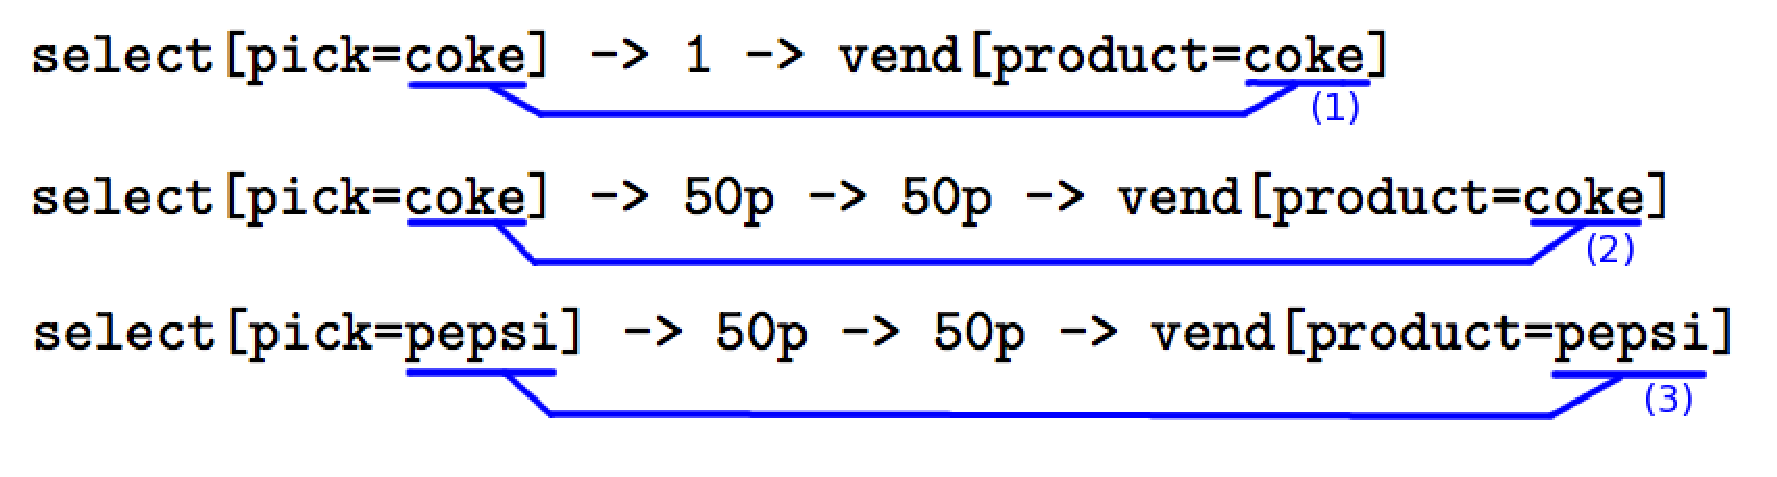
\includegraphics[width=14cm]{figures/efsm/intratracedeps.eps}
\caption{Some traces of the vending machine}
\label{fig:intras}
\end{center}
\end{figure}

Whenever a trace is added to the system it is analysed for instances of data re-use. These are referred to as Intra-Trace Dependencies. The Athena implementation is able to identify data re-use of both complete values, such as those shown in \fig{fig:intras}, or substrings of values. 

%[FIXME move later? Or drop because its not used in the case study?] In the latter case the guard and output expression language supports the operators $match$ and $get$. The $match$ can test whether a string matches a general pattern --- containing a variable value surrounded by a specific prefix and suffix, but not necessarily at a given position\footnote{This was designed to support HTTP style key-value pairings, where the order of pairings is not enforced but their syntax makes them identifiable.}. The $get$ operator is used in output and update computations and retrieves the variable value from such a pattern. For example, in the event that $i_1 = "key=xyz;"$ the expression $match("key=",";",r_1)$ would evaluate to $true$, while the expression $get("key=",";",r_1)$ would evaluate to the string $"xyz"$. The application of these operators is still experimental and is not applied extensively in the examples.

The formal structure of an Intra-Trace Dependency is as a triple containing the value that was reused and two further triples identifying the event and parameter of the first and second instance of the value. For example, the instance of re-use identified in red in the first trace in \fig{fig:intras} would be represented as $("coke",(1,i,1),(4,o,1))$, representing that the re-used value is $"coke"$ and it is used in the 1st event as input 1, and in the 4th event as output 1.

However, these instances of data re-use may be simple coincidences --- such as the blue arrows in \fig{fig:intras} --- so the Athena implementation takes no action except to store all the Intra-Trace Dependencies for each trace. In the same way that Evidence Based State Merging is used to choose control flow states to merge, so \emph{evidence} is required before patterns of data re-use are codified in the EFSM model. Evidence is provided when the patterns of data re-use \emph{align}. As control flow states are merged, so the transitions of different traces can become attached to the same state. The Athena implementation tracks the original trace and event number that was the source of all the transitions in the original PTA. As transitions are moved onto the same state the Intra-Trace Dependencies of these underlying traces are checked. Where there are multiple Intra-Trace Dependencies whose first elements are now attached to the same state, whose second elements are attached to the same state, and which have matching patterns of I/O use this forms an Inter-Trace Dependency. 

\begin{figure}[h]
\begin{center}
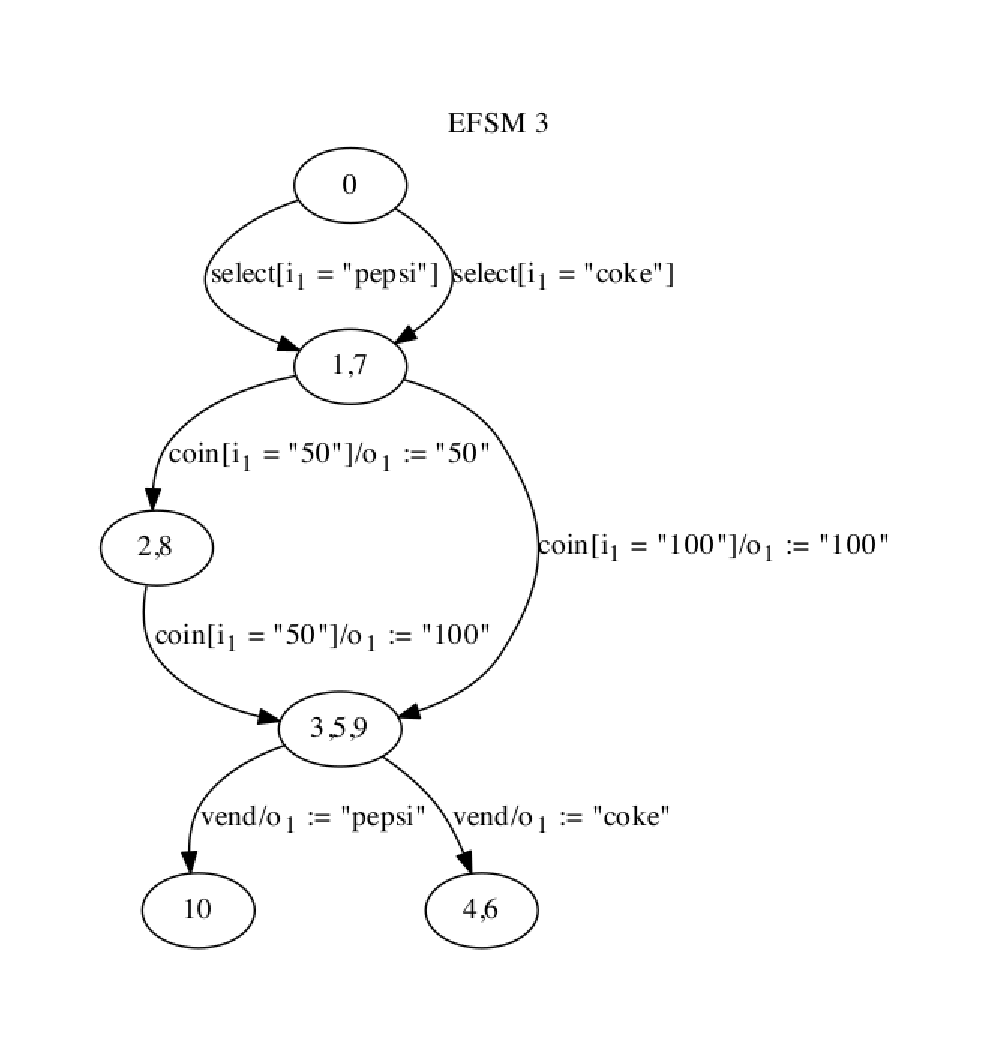
\includegraphics[width=12cm]{figures/efsm/predata.eps}
\caption{The state machine after some merging}
\label{fig:predata}
\end{center}
\end{figure}

An example of this can be seen in \fig{fig:predata}, where the re-use of the strings $"coke"$ and $"pepsi"$ has aligned --- it is first encountered on the transitions out of state 0, and then again on the transitions out of state "3,5,9". It is significant that often (as in this case) the values themselves differ between traces --- it is the \emph{pattern of re-use} that has been identified. This provides evidence that the underlying system is re-using the data at these two points, and so it is necessary to add the data to the data state of the EFSM. 

At this point the Athena implementation adds a fresh register to the EFSM data state and produces a new transition based on the first transitions in the pattern but which generalises the guard to no longer require the exact value from one instance, and which updates the fresh register with whatever value is observed. A second transition is added in the second position that generalises the second pattern and makes use of the fresh register. These two new transitions will necessarily be generalisations of the original transitions, and this may well cause the Athena implementation's non-determinism resolution procedures to merge the original transitions into this, and --- possibly --- to merge some states that now seem identical.

\begin{figure}[h]
\begin{center}
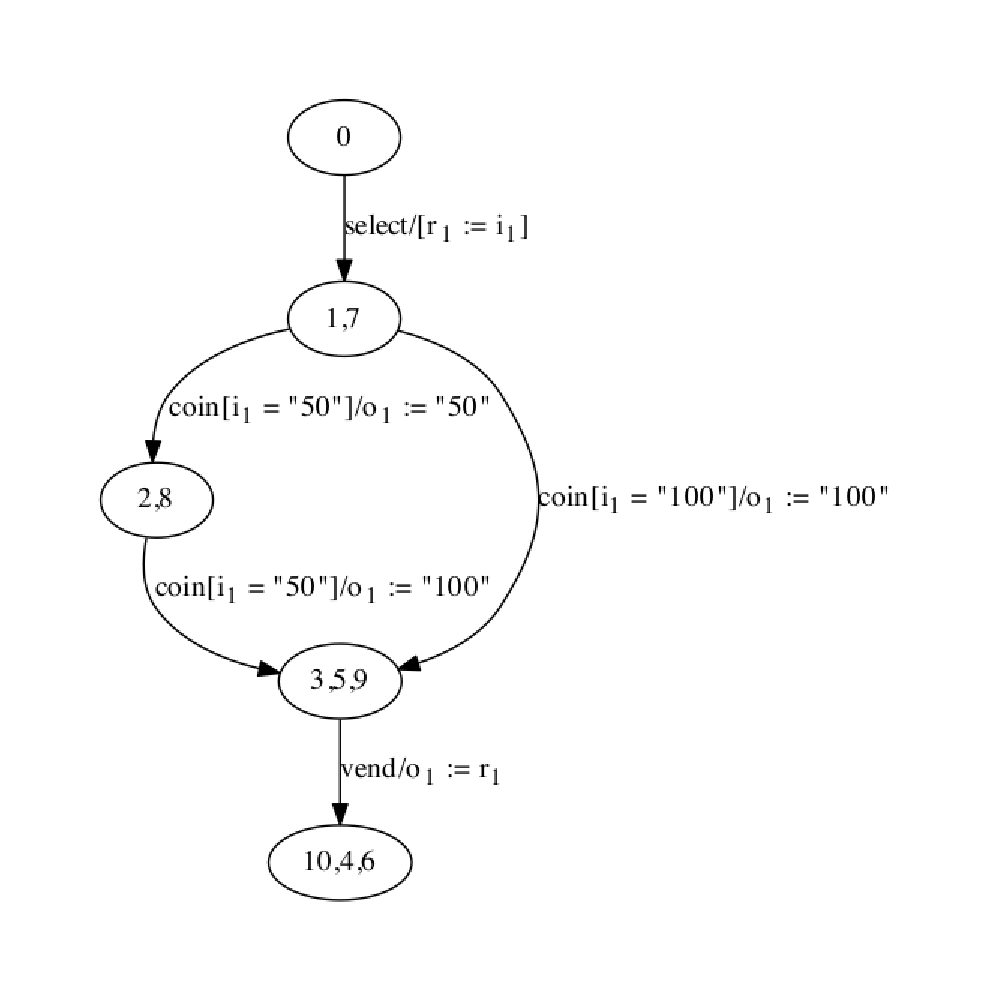
\includegraphics[width=12cm]{figures/efsm/data.eps}
\caption{A EFSM with a data register added and used}
\label{fig:data}
\end{center}
\end{figure}

The resulting vending machine diagram is shown in \fig{fig:data}, where the data register $r_1$ has been added, along with an update function to store the value of $i_1$ and then re-use it to set the value of $o_1$ later. The standard Evidence Driven State Merging process can now repeat on this machine, and will likely merge further states, since the general expression $o_1 := r_1$ will be scored as highly similar to any specific instances of outputs, such as $o_1 := "fanta"$.

\subsubsection{Contradictory Transitions}
\label{Splitting}

The previous sections have discussed how the inference process generalises from the observed instances to build an EFSM model that explains all the observed traces and can predict future values. However, with iterative learning it is possible that a trace observed later may contradict the EFSM model. It can do this by following a transition in apparent violation of its guard, producing a different output from that computed by the EFSM, or by performing an action that should not be possible from this control flow state.

In these cases either transitions or control flow states need to be \emph{split} to incorporate the new data without contradiction. Ideally, such contradictions can be resolved by re-running the genetic programming described in \sect{Generalisation} incorporating the new information. This can produce improved guard expressions, since more information provides a more accurate fitness function for the evolutionary process. 

However, where the contradiction at a given control flow state cannot be resolved over the data this must be the result of control flow states being merged in the model that are different states of the true system. In this case the states need to be split, but it may not be the state at which the contradiction appears that is the state that was incorrectly merged, the true system may have branched several events earlier. To unravel this, the Athena implementation uses the retained trace and event data stored in the transitions and backtracks along each of the traces involved in the contradiction. The immediately preceding events maybe completely identical (in both event and data) so the backtracking continues until there is an observable difference. At this point the two explicit transitions are re-added to the model and the subsequent traces re-added in the style of the original PTA. The merging and generalisation process can then continue, and that will re-merge any states that are still compatible.

It is important that this processes is performed over the original trace information and not over the transitions in the generalised models because loops in the EFSM can obscure the true position of the contradiction.

\section{Conclusions}
\label{concs}

The work reported here shows that we are able to automate the process of parametrising QuickCheck state machines -- that 
is extended finite-state machines -- in line with different versions or configurations of a system.

It also shows that we are able to transform non-parametric models into parametric ones by providing refactoring support in Wrangler for an ``introduce behaviour'' refactoring, as well as to provide decision support for parametrisation introduction by implementing a ``diff'' mechanism for models; moreover, we have shown how these facilities work in practice in a set of case studies. While the mechanism can be used in completely automatic mode, we have demonstrated in the case studies that some manual tuning can improve the style and comprehensibility of the resulting  parametric system. In looking at the DETS/ETS example we have shown that the process is scalable beyond purely ``toy'' examples to systems that are in everyday use by Erlang programmers.

Finally we have shown that the process of deriving an \emph{extended} finite state machine from a set of traces for the system is achievable through an extension on classical techniques and some search-based programming. We have also demonstrated the effectiveness of the approach in the pilot study reported in detail in Deliverable D6.6.

In both strands of research we have delivered tools and techniques that accomplish not only the original goals of the project but also wider results that will be of value in the wider programming, modelling and property-based testing communities.
